\documentclass[aspectratio=141]{beamer}
\usepackage{amsmath}
\usepackage{bbm}
\usepackage{stmaryrd}
\usepackage{ebproof}
\usepackage{tikz-cd}
\usepackage{array}
\usepackage{appendixnumberbeamer}

%\usetheme{Rochester}
\useoutertheme[left,height=0pt,width=0.14\paperwidth]{sidebar}
\usecolortheme{orchid}
\usecolortheme{dolphin}
\useinnertheme[shadow=true]{rounded}
\usefonttheme[onlylarge]{structurebold}
\newlength{\layerwidth}
\setlength{\layerwidth}{.4\textwidth}
\setlength{\parskip}{1ex}

% Commands {{{
\newcommand{\kw}[1]{\ensuremath{ \mathrm{#1} }}
\newcommand{\bdot}{\boldsymbol{\cdot}}
\newcommand{\htr}[3]{{ {#1} \mathbbm{\{} {#2} \mathbbm{\}} {#3} }}
\newcommand{\ljg}[5]{{#2} \vdash^{#1}_{#3} {#4} : {#5}}
\newcommand{\jg}[4]{\ljg{}{#1}{#2}{#3}{#4}}
\newcommand{\fme}{\textbf{J\'er\'emie~Koenig}}
\newcommand{\me}{\textbf{J. K.}}
\newcommand{\module}[1]{\framebox[\layerwidth]{\ensuremath{#1}} }
\newcommand{\smodule}[1]{\framebox[0.435\layerwidth]{\ensuremath{#1}} }
\newcommand{\gmodule}[1]{\framebox[0.435\layerwidth]{\ensuremath{#1}} }

\AtBeginSection{
  \frame{\sectionpage}
}

\addtobeamertemplate{navigation symbols}{}{%
  \usebeamerfont{footline}%
  \usebeamercolor[fg]{footline}%
  \hspace{1em}%
  \raisebox{0.5ex}{\insertframenumber/\inserttotalframenumber}
}

% Pictures %{{{

\newcommand{\rotpic}[2]{%
  \begin{tikzpicture}[scale=0.4]
    \draw (-4,-1) rectangle (4,1);
    \node (x) at (0,0) {$#1$};
    \draw[->] (-3, -1) -- (-3, -2);
    \node[anchor=base] at (-3, -3) {\small $\kw{deq}$};
    \draw[<-] (-1.3, -1) -- (-1.3, -2);
    \node[anchor=base] at (-1.3, -3) {$#2$};
    \draw[->] (1, -1) -- (1, -2);
    \node[anchor=base] at (1, -3) {\small $\kw{enq}(#2)$};
    \draw[<-] (3, -1) -- (3, -2);
    \node[anchor=base] at (3, -3) {$*$};
    \draw[->] (4,0) -- node[above] {$#2$} (6,0);
  \end{tikzpicture}%
}

\newcommand{\deqpic}[3]{%
  \begin{tikzpicture}[scale=0.4]
    \draw (-4,-1) rectangle (4,1);
    \node (x) at (0,0) {$#1$};
    \draw[->] (-3, -1) -- (-3, -2);
    \node[anchor=base] at (-3, -3) {\small $\kw{inc}_1$};
    \draw[<-] (-1.3, -1) -- (-1.3, -2);
    \node[anchor=base] at (-1.3, -3) {$#2$};
    \draw[->] (1, -1) -- (1, -2);
    \node[anchor=base] at (1, -3) {\small $\kw{get}[#2]$};
    \draw[<-] (3, -1) -- (3, -2);
    \node[anchor=base] at (3, -3) {$#3$};
    \draw[->] (4,0) -- node[above] {$#3$} (6,0);
  \end{tikzpicture}%
}

%}}}

\title[Refinement-Based Game Semantics]%{{{
  {Refinement-Based Game Semantics \\ for Certified Components}
\author{J\'er\'emie Koenig}
\institute{Advisor: Zhong Shao \\ Yale University}
\date{July 20, 2020}
%}}}

\begin{document}

\begin{frame}
\titlepage
\end{frame}

\setbeamertemplate{bibliography entry location}{}
\setbeamertemplate{bibliography entry title}{}
%\setbeamertemplate{bibliography item}[online]
\setbeamerfont{bibliography entry author}{size=\footnotesize}

%\begin{frame}[fragile]{CertiKOS} %{{{
%CertiKOS is a certified operating system kernel:
%its assembly code comes with a computer-checked,
%mathematical proof of correctness.
%
%We show the following \emph{contextual refinement} property:
%\[
%    \forall P \,.\,
%        \llbracket P \oplus \kw{CertiKOS} \rrbracket_{\kw{x86}}
%        \sqsubseteq
%        \llbracket P \rrbracket_{\kw{TSyscall}}
%\]
%Schematically:
%\[
%  \begin{prooftree}
%    \hypo{P}
%    \infer1[$\kw{TSysCall}$]{\text{\module{ \kw{CertiKOS} }} }
%    \infer1[$\kw{x86}$]{}
%  \end{prooftree}
%\]
%If the layer interfaces are seen as \emph{languages},
%adding the code of \kw{CertiKOS} to a program can be seen as
%a special case of \emph{certified compilation}.
%\end{frame}
%%}}}
%
%\begin{frame}{Layered decomposition} %{{{
%Because contextual refinement is transitive,
%we can split \kw{CertiKOS} into \emph{layers}:
%\[
%    \kw{CertiKOS} =
%        M_\kw{Container} \oplus M_\kw{ALInit} \oplus \ldots \oplus M_\kw{SysCall}
%\]
%\[
%  \begin{prooftree}
%    \hypo{}
%    \infer1[$\kw{TSysCall}$]{\module{M_\kw{SysCall} }}
%    \infer1[$\kw{TDispatch}$]{\vdots}
%    \infer1[$\kw{MALInit}$]{\module{M_\kw{ALInit} }}
%    \infer1[$\kw{MContainer}$]{\module{M_\kw{Container} }}
%    \infer1[$\kw{MBoot}$]{}
%  \end{prooftree}
%\]
%
%At each layer,
%a \emph{module} $M$ implements
%an \emph{overlay interface} $L_2$ in terms of
%an \emph{underlay interface} $L_1$.
%\end{frame}
%%}}}
%
%\begin{frame}{DeepSpec: Certified heterogenous systems}
%\end{frame}
%
%\begin{frame}{Modeling open systems}
%\end{frame}

%\section{Introduction} {{{

\begin{frame}{Scaling up certified software} %{{{
  Certified software this past decade:
  \begin{itemize}
    \item C compiler (CompCert) and program logic (VST)
    \item Operating system kernel (CertiKOS), file system (FSCQ)
    \item Processor designs (Bluespec), \ldots
  \end{itemize}

  \pause
  To scale up verification further, we need a compositional glue:
  \begin{itemize}
    \item Heterogenous: general-purpose model, embed various components
    \item Composition and abstraction: high-level algebraic structures
  \end{itemize}
  %The DeepSpec project seeks to build:
  %\begin{itemize}
  %  \pause \item Large-scale, heterogenous systems
  %  \pause \item Certified end-to-end in a general-purpose proof assistant
  %  \pause \item Constructed from off-the-shelf certified components.
  %\end{itemize}
\end{frame}
%}}}

\begin{frame}{Case study: CertiKOS} %{{{
  Software systems use abstraction layers. In CertiKOS:
  \[
    \begin{prooftree}
      \hypo{C}
      \infer1[$L_n$]{\fbox{$\qquad M_n \qquad$}}
      \infer1[$L_{n-1}$]{\vdots}
      \infer1[$L_1$]{\fbox{$\qquad M_1 \qquad$}}
      \infer1[$L_0$]{}
    \end{prooftree}
    \qquad
    \vcenter{\hbox{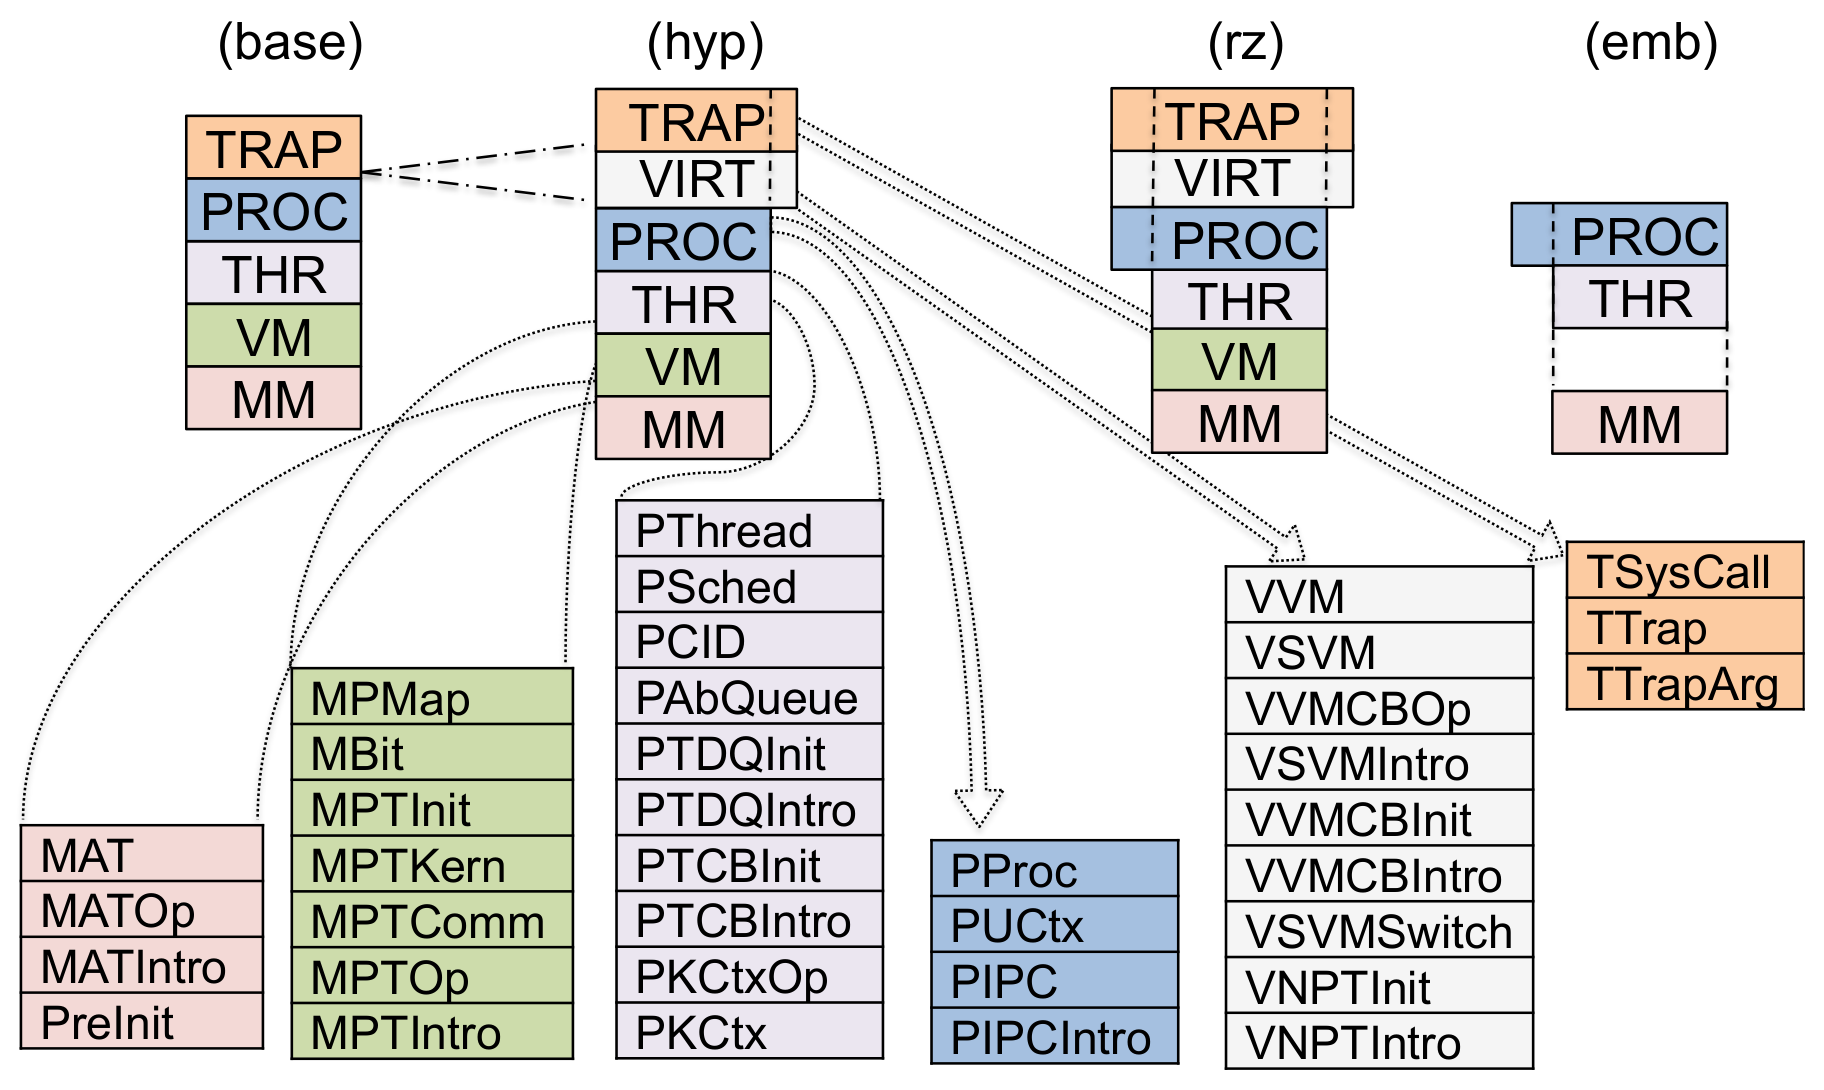
\includegraphics[scale=0.55]{layers} }}
  \]

  \pause
  Our verification effort uses
  \emph{certified abstraction layers}:
  \[
    \begin{prooftree}
      \hypo{C}
      \infer1[$L_2$]{\begin{array}{c}R \\ \fbox{$\qquad M \qquad$}\end{array}}
      \infer1[$L_1$]{}
    \end{prooftree}
    \qquad
    \begin{array}{c}
      \fbox{$L_1 \vdash M : L_2$} \\[1em]
      \forall C \: \bdot \:
      \llbracket C \rrbracket_{L_2} \le_R
      \llbracket C \oplus M \rrbracket_{L_1}
    \end{array}
  \]
%
%  \pause
%  Using transitivity we achieve compositional verification:
%
%    \qquad
%    \begin{array}{r@{\:}l}
%      \forall C \: \bdot &
%      \llbracket C \rrbracket_\kw{TSyscall} \\
%      \sqsubseteq &
%      \llbracket C \oplus M_n \rrbracket_\kw{TTrap} \\
%      \vdots &
%      \\
%      \sqsubseteq &
%      \llbracket C \oplus M_n \oplus \cdots \oplus M_2
%      \rrbracket_\kw{MATInit} \\
%      \sqsubseteq &
%      \llbracket C \oplus M_n \oplus \cdots \oplus M_2 \oplus M_1
%      \rrbracket_\kw{MBoot}
%    \end{array}
\end{frame}
%}}}

\begin{frame}{Great research not used in large-scale verification} %{{{
  \textbf{Good news:}
  There is lot of research that we can draw from!

  \textbf{Bad news:}
  Few applications to
  large-scale verification.

  \vfill
  \begin{center}
    \begin{tabular}{cc}
      \hline
      Semantics research &
      Typical verification project
      \\
      \hline
      \\[-1ex]
      %\parbox{.4\textwidth}{
      %  \centering
      %  Game semantics \\ Linear logic
      %} &
      \parbox{10em}{\centering Game semantics \\ Linear logic} &
      Transition systems \\[1em]
      Refinement calculus &
      Simulations \\[1em]
      Logical relations &
      Hoare logic \\[1em]
      Algebraic effects &
      Closed systems \\[1em]
      \hline
    \end{tabular}
  \end{center}
\end{frame}
%}}}

\begin{frame}{Why this gap?} %{{{
  Challenges:
  \begin{itemize}
    \item Sophisticated models hard to mechanize in proof assistants
    \item Not clear how these techniques can work together
  \end{itemize}

  For example:
  \begin{itemize}
    \item Game semantics: not much emphasis on refinement
    \item Refinement calculus: imperative programming and specification
  \end{itemize}
\end{frame}  
%}}}

\begin{frame}{Contributions} %{{{
We combine various paradigms to introduce:
\begin{center}
\textbf{Refinement-Based Game Semantics}
\end{center}

\pause
Our models provide:
\begin{itemize}
  \item \textbf{Compositionality:}
    categories with symmetric monoidal structures
  \item \textbf{Refinement:}
    uniform treatment of programs and specifications
  \item \textbf{Dual nondeterminism:}
    for expressivity and data abstraction
  %\item \emph{Symmetric monoidal categories} for compositionality;
  %\item \emph{Strategy specifications} to support stepwise refinement;
  %\item \emph{Dual nondeterminism} for open systems and data abstraction.
\end{itemize}

\pause
Key insights:
\begin{itemize}
  \item Reinterpret strategies as inherently nondeterministic
  \item Upgrade to dual nondeterminism and lift all restrictions
\end{itemize}

%Based on a new approach to
%nondeterminism in game semantics,
%we introduce \emph{refinement-based game semantics}:
%%syntesizing techniques from game semantics and stepwise refinement,
%%and apply them to simple game models:
%\pause
%\begin{itemize}
%  \item Games are first-order signatures $E, F$;
%  \item \emph{Strategy specifications} are morphisms $f : E \rightarrow F$;
%  \item They are equipped with complete lattices,
%    representing \emph{dual nondeterminism}
%\end{itemize}

%\pause
%The result is a very expressive framework,
%which nevertheless remains simple enough to
%formalize in a proof assistant.

%\pause
%In particular,
%our models are rich enough to embed
%certified abstraction layers
%and a compositional semantics for CompCert.
\end{frame}
%}}}

\begin{frame}{Outline} %{{{
  \tableofcontents
\end{frame}
%}}}

%}}}

\section{Overview} %{{{

\begin{frame}{Capturing patterns in layers} %{{{
  \begin{center}
    \small
    \begin{tabular}{lc@{\qquad}c}
      \rule[-2em]{0pt}{4em}
      Elementary proof &
      \rule{0pt}{5ex}
      {\begin{prooftree}
        \hypo{\kw{CP}(L, R, \kappa, \sigma)}
        \infer1{\jg{L}{R}{i \mapsto \kappa}{i \mapsto \sigma}}
      \end{prooftree}} &
      \begin{minipage}[c]{.1\textwidth}
      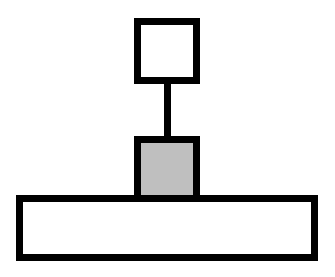
\includegraphics[scale=.15]{fig/element}
      \end{minipage} \\
      \rule[-2em]{0pt}{4em}
      Horizontal composition &
      \rule{0pt}{5ex}
      {\begin{prooftree}
        \hypo{\jg{L}{R}{M_1}{L_1}}
        \hypo{\jg{L}{R}{M_2}{L_2}}
        \infer2{\jg{L}{R}{M_1 \oplus M_2}{L_1 \oplus L_2}}
      \end{prooftree}} &
      \begin{minipage}[c]{.1\textwidth}
      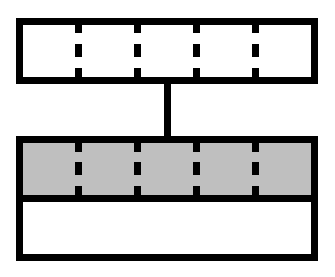
\includegraphics[scale=.15]{fig/hcomp}
      \end{minipage} \\
      \rule[-2em]{0pt}{4em}
      Vertical composition &
      \rule{0pt}{6ex}
      {\begin{prooftree}
        \hypo{\jg{L_1}{R}{M}{L_2}}
        \hypo{\jg{L_2}{S}{N}{L_3}}
        \infer2{\jg{L_1}{R \circ S}{M \oplus N}{L_3}}
      \end{prooftree}} &
      \begin{minipage}[c]{.1\textwidth}
      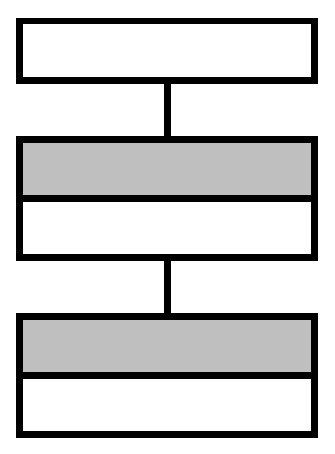
\includegraphics[scale=.15]{fig/vcomp}
      \end{minipage} \\
      \rule[-2em]{0pt}{4em}
      Soundness &
      \rule{0pt}{5ex}
      {\begin{prooftree}
        \hypo{\jg{L_1}{R}{M}{L_2}}
        \infer1{\forall P . \llbracket P \oplus M \rrbracket_{L_1} \sqsubseteq
                      \llbracket P \rrbracket_{L_2}}
      \end{prooftree}} &
      \tiny
      \hspace{-1.5em}
      $C[-] \sqsubseteq C[-]$
    \end{tabular}
  \end{center}
  %\vfill
  \begin{thebibliography}{10}
    \bibitem{popl15}
      Ronghui~Gu, \fme,
      Tahina~Ramananandro, Zhong~Shao,
      Xiongnan~(Newman)~Wu, Shu-Chun~Weng, Haozhong~Zhang.
      \newblock \\
      Deep Specifications and Certified Abstraction Layers.
      \newblock
      POPL '15.
  \end{thebibliography}
\end{frame}
%}}}

\begin{frame}{Automating relational reasoning in Coq} %{{{
  CompCert semantics are complicated.
  But our soundness can be simple:
  \begin{center}
    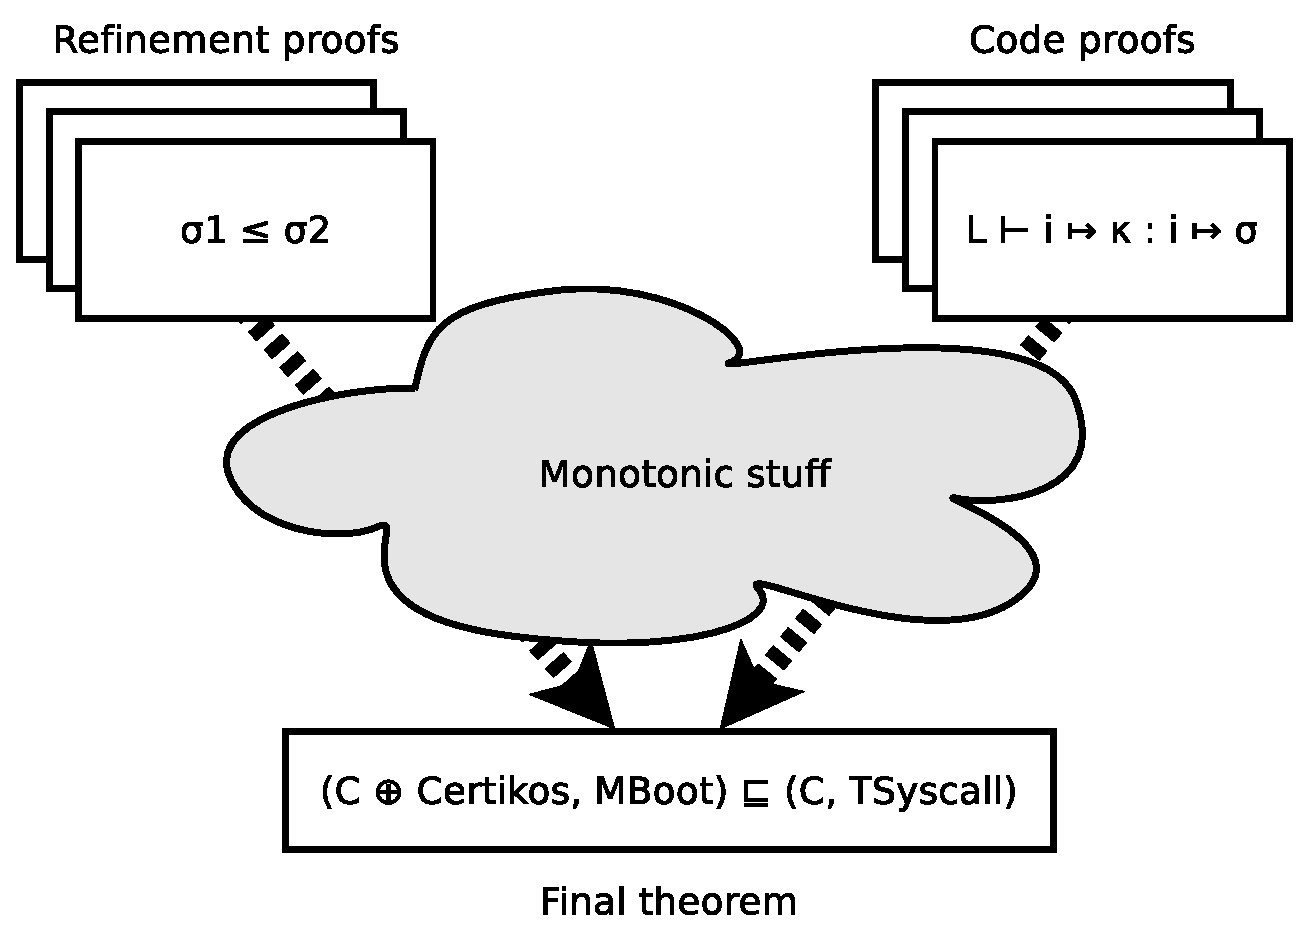
\includegraphics[scale=0.35]{fig/overview}
  \end{center}
  \begin{thebibliography}{10}
    \setbeamertemplate{bibliography item}[online]
    \bibitem{coqrel-code}
      \url{https://github.com/CertiKOS/coqrel}
    \setbeamertemplate{bibliography item}[default]
    \bibitem{coqrel}
      \fme.
      \newblock
      A Coq Library for Binary Logical Relations.
      \newblock
      CoqPL '16.
  \end{thebibliography}
\end{frame}
%}}}

\begin{frame}{Concurrent layers and oracles} %{{{
  Thread linking in concurrent CertiKOS:
  \[
    \begin{prooftree}
      \hypo{\smodule{\kw{TSyscall} }}
      \infer1{\vdots}
      \infer1{\smodule{\kw{PThread} }}
      \hypo{\gmodule{\kw{TSyscall} }}
      \infer1{\color{gray}\vdots}
      \infer1{\gmodule{\kw{PThread} }}
      \infer2{\module{\kw{PThread} }}
      \infer1{\vdots}
      \infer1{\module{\text{Per-core services} }}
    \end{prooftree}
  \]
  \vfill
  \begin{thebibliography}{10}
    \bibitem{ccal}
      Ronghui~Gu, Zhong~Shao, Jieung~Kim, Xiongnan~(Newman)~Wu,
      \me, Vilhelm~Sj\"oberg, Hao~Chen,
      David~Costanzo, Tahina~Ramananandro.
      \newblock \\
      Certified Concurrent Abstraction Layers.
      \newblock
      PLDI '18.
  \end{thebibliography}
\end{frame}
%}}}

\begin{frame}{Refinement-based game semantics} %{{{
  \vfill
  \begin{thebibliography}{10}
    \setbeamertemplate{bibliography item}[online]
    \bibitem{rbgs-code}
      \url{https://github.com/CertiKOS/rbgs}
    \setbeamertemplate{bibliography item}[default]
    \bibitem{rbgs-cal}
      \fme, Zhong Shao.
      \newblock \\
      Refinement-Based Game Semantics for Certified Abstraction Layers.
      \newblock
      LICS '20.
  \end{thebibliography}
\end{frame}
%}}}

\begin{frame}{CompCertO} %{{{
  \vfill
  \begin{thebibliography}{10}
    \setbeamertemplate{bibliography item}[online]
    \bibitem{compcerto-code}
      \url{https://github.com/CertiKOS/compcert/tree/compcerto}
    \setbeamertemplate{bibliography item}[default]
    \bibitem{compcerto}
      \fme, Zhong Shao.
      \newblock \\
      CompCertO: Compiling Certified Open C Components.
      \newblock
      Submitted.
  \end{thebibliography}
\end{frame}
%}}}

\begin{frame}{Other work} %{{{
  \begin{thebibliography}{10}
    \bibitem{otf}
      Joan Feigenbaum, \fme.
      \newblock \\
      On the Feasability of
      a Technological Response to the Surveillance Morass.
      \newblock \\
      Cambridge Int'l Workshop on Security Protocols 2014.
    \bibitem{rbp}
      Omid Alipourfard, Jiaqi Gao, \me,
      Chris~Harshaw, Amin~Vahdat, Minlan~Yu.
      \newblock
      Risk-based Planning of Network Changes in Evolving Data Centers.
      \newblock \\
      SOSP '19.
  \end{thebibliography}
\end{frame}
%}}}

%}}}

\section{Certified abstraction layers} %{{{

\begin{frame}{First-order signatures as games} %{{{
  \begin{definition}[Signature]
  \[
    E = \{ m_1 \mathop{:} N_1, \ldots, m_j \mathop{:} N_j \}
  \]
  Each $m_i \mathop{:} N_i \in E$ is a \emph{question},
  with $n_i \in N_i$ a corresponding \emph{answer}.
  \end{definition}
  \pause
  \begin{example}[Bounded queue]
    We implement a queue using an array and two counters:
    \begin{gather*}
      E_\kw{q} := \{
        \kw{enq}[v] \mathop{:} \mathbbm{1}, \:
        \kw{deq} \mathop{:} V \mid
        v \in V \}
      \\
      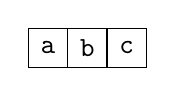
\begin{tikzpicture}[scale=0.5]
        \draw (0,0) grid (3,1);
        \node at (0.5,0.5) {$\mathtt{a}$};
        \node at (1.5,0.5) {$\mathtt{b}$};
        \node at (2.5,0.5) {$\mathtt{c}$};
      \end{tikzpicture}
      \\[1ex]
      E_\kw{a} := \{
        \kw{get}[i] {:} V, \:
        \kw{set}[i,v] {:} \mathbbm{1}, \:
        \kw{inc}_1 {:} \mathbb{N}, \:
        \kw{inc}_2 {:} \mathbb{N}
        \mid i \in \mathbb{N}, v \in V \} \\
      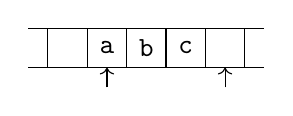
\begin{tikzpicture}[scale=0.5]
        \draw (-0.5,0) grid (5.5,1);
        \node at (1.5,0.5) {$\mathtt{a}$};
        \node at (2.5,0.5) {$\mathtt{b}$};
        \node at (3.5,0.5) {$\mathtt{c}$};
        \draw[->] (1.5,-0.5) -- (1.5,0);
        \draw[->] (4.5,-0.5) -- (4.5,0);
      \end{tikzpicture}
    \end{gather*}
  \end{example}
\end{frame}
%}}}

\begin{frame}{Layer interfaces}
\[
    S \rightarrow \mathcal{P}^1(S \times V)
\]
\end{frame}

\begin{frame}{Client code}

\end{frame}

\begin{frame}{Layer implementation}

\end{frame}

\begin{frame}{Correctness}

\end{frame}

\begin{frame}{Vertical composition}

\end{frame}

\begin{frame}{Horizontal composition}

\end{frame}

\begin{frame}{Conclusion}

\end{frame}

%}}}

\section{Refinement-based game semantics} %{{{

%
%\begin{frame}[fragile]{Angelic and demonic nondeterminism} %{{{
%  Hoare logic and axiomatic semantics use
%  \emph{correctness statements}:
%  \begin{gather*}
%    \fbox{$\htr{P}{C}{Q}$} \\[1ex]
%    \xrightarrow{k} \fbox{$C$} \xrightarrow{k'} \\
%    P(k) \Rightarrow Q(k')
%  \end{gather*}
%
%  \pause
%  Two ways to add nondeterministic choice:
%  \onslide<2->
%  \only<1-2>{
%    \begin{gather*}
%      \fbox{$C_1 \sqcup C_2$}
%      \\[1ex]
%      {\begin{prooftree}
%        \hypo{\htr{P}{C_1}{Q}}
%        \infer1{\htr{P}{C_1 \sqcup C_2}{Q}}
%      \end{prooftree}}
%      \qquad
%      {\begin{prooftree}
%        \hypo{\htr{P}{C_2}{Q}}
%        \infer1{\htr{P}{C_1 \sqcup C_2}{Q}}
%      \end{prooftree}}
%    \end{gather*}
%  }
%  \only<3>{
%    \begin{gather*}
%      \fbox{$C_1 \sqcap C_2$}
%      \\[1ex]
%      {\begin{prooftree}
%        \hypo{\htr{P}{C_1}{Q}}
%        \hypo{\htr{P}{C_2}{Q}}
%        \infer2{\htr{P}{C_1 \sqcap C_2}{Q}}
%      \end{prooftree}}
%    \end{gather*}
%  }
%\end{frame}
%%}}}
%

\begin{frame}{Refinement and nondeterminism} %{{{
  \begin{block}{Stepwise refinement}
  Key idea: uniform treatment of programs and specifications
  \begin{gather*}
    \fbox{$C_1 \sqsubseteq C_2$} \\[1ex]
    \htr{P}{C}{Q} \: \Leftrightarrow \:
      \langle P | Q \rangle \sqsubseteq C \\
    S \sqsubseteq C_1 \sqsubseteq \cdots \sqsubseteq C_n
  \end{gather*}
  \end{block}
  \pause
  \onslide<2->%
  \begin{block}{Nondeterminism in specifications}
  \only<1-2>{
    \begin{tikzpicture}[overlay]
      \node[anchor=north west] at (0,0) {
\includegraphics[scale=0.065]{angel}};
    \end{tikzpicture}
    \begin{gather*}
      \fbox{$S_1 \sqcup S_2 \sqsubseteq C$}
      \\[1ex]
      {\begin{prooftree}
        \hypo{S_1 \sqsubseteq C}
        \hypo{S_2 \sqsubseteq C}
        \infer2{S_1 \sqcup S_2 \sqsubseteq C}
      \end{prooftree}}
    \end{gather*}
    \vspace{1ex}
  }%
  \only<3>{
    \flushright%
    \begin{tikzpicture}[overlay]
      \node[anchor=north east] at (0,0.3)
        {
\includegraphics[scale=0.07]{demon}};
    \end{tikzpicture}
    \begin{gather*}
      \fbox{$S_1 \sqcap S_2 \sqsubseteq C$}
      \\[1ex]
      {\begin{prooftree}
        \hypo{S_1 \sqsubseteq C}
        \infer1{S_1 \sqcap S_2 \sqsubseteq C}
      \end{prooftree}}
      \qquad
      {\begin{prooftree}
        \hypo{S_2 \sqsubseteq C}
        \infer1{S_1 \sqcap S_2 \sqsubseteq C}
      \end{prooftree}}
    \end{gather*}
    \vspace{1ex}
  }%
  \end{block}

%  \only<1-3>{
%    In programs, angelic and demonic choices work as before:
%  }%
%  \only<1-2>{
%    \begin{gather*}
%      \fbox{$S \sqsubseteq C_1 \sqcup C_2$}
%      \\[1ex]
%      {\begin{prooftree}
%        \hypo{S \sqsubseteq C_1}
%        \infer1{S \sqsubseteq C_1 \sqcup C_2}
%      \end{prooftree}}
%      \qquad
%      {\begin{prooftree}
%        \hypo{S \sqsubseteq C_2}
%        \infer1{S \sqsubseteq C_1 \sqcup C_2}
%      \end{prooftree}}
%    \end{gather*}
%  }%
%  \only<3>{
%    \begin{gather*}
%      \fbox{$S \sqsubseteq C_1 \sqcap C_2$}
%      \\[1ex]
%      {\begin{prooftree}
%        \hypo{S \sqsubseteq C_1}
%        \hypo{S \sqsubseteq C_2}
%        \infer2{S \sqsubseteq C_1 \sqcap C_2}
%      \end{prooftree}}
%    \end{gather*}
%  }%
%  \only<4-5>{%
%    In specifications, the point of view is reversed:
%  }%
%  \only<4>{
%    \begin{gather*}
%      \fbox{$S_1 \sqcup S_2 \sqsubseteq C$}
%      \\[1ex]
%      {\begin{prooftree}
%        \hypo{S_1 \sqsubseteq C}
%        \hypo{S_2 \sqsubseteq C}
%        \infer2{S_1 \sqcup S_2 \sqsubseteq C}
%      \end{prooftree}}
%    \end{gather*}
%  }%
%  \only<5>{
%    \begin{gather*}
%      \fbox{$S_1 \sqcap S_2 \sqsubseteq C$}
%      \\[1ex]
%      {\begin{prooftree}
%        \hypo{S_1 \sqsubseteq C}
%        \infer1{S_1 \sqcap S_2 \sqsubseteq C}
%      \end{prooftree}}
%      \qquad
%      {\begin{prooftree}
%        \hypo{S_2 \sqsubseteq C}
%        \infer1{S_1 \sqcap S_2 \sqsubseteq C}
%      \end{prooftree}}
%    \end{gather*}
%  }%
%  Then:
%  \begin{itemize}
%    \item \emph{Transitivity} enables incremental derivation
%    \item \emph{Monotonicity} enables congruent refinement
%    \item \emph{Nondeterminism} enhances expressivity for specifications
%    \item $\sqsubseteq, \sqcup, \sqcap$ work together
%      as a \emph{distributive lattice}
%  \end{itemize}
\end{frame}
%}}}

\begin{frame}{Dual nondeterminism and distributive lattices} %{{{
  $\sqsubseteq$, $\sqcup$, $\sqcap$ work together as a
  \emph{completely distributive lattice}:
  \begin{itemize}
    \item Associativity of $\sqcup$, $\sqcap$: insensitive to branching
    \item Complete distributivity:
      \[
        \bigsqcup_{i \in I} \bigsqcap_{j \in J_i} x_{i,j} =
        \bigsqcap_{f \in \prod_{i \in I} J_i \:\:}
          \bigsqcup_{i \in I} \: x_{i,f(i)}
      \]
      Angelic and demonic choice also commute with each other
    \item Refinement increases $\sqcup$, decreases $\sqcap$
  \end{itemize}
\end{frame}
%}}}

\begin{frame}{Example: nondeterministic functions} %{{{
A function $f : \mathbb{Z} \rightarrow \mathbb{Z}$
can be seen as a simple system:
\[
  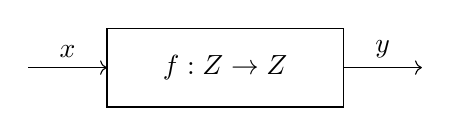
\begin{tikzpicture}[scale=0.5]
    \draw (-3, -1) rectangle (3, 1);
    \node at (0,0) {$f : \mathbb{Z} \rightarrow \mathbb{Z}$};
    \draw[->] (-5,0) -- node[above] {$x$} (-3,0);
    \draw[->] (3,0) -- node[above] {$y$} (5,0);
  \end{tikzpicture}
\]
The specification $x \mapsto y$ means:
\begin{quotation}
\vspace{1ex}
  When the input is $x$, the output must be $y$.
\end{quotation}

\pause
The function $f(x) := 2x$ statisfies the specifications:
\[
  \only<3->{\begin{tikzpicture}[overlay]
    \node[left] at (-0.5,0) {
\includegraphics[scale=0.05]{angel-only}};
  \end{tikzpicture}}
  0 \mapsto 0 \pause \:\:\sqsubseteq\:\:
  0 \mapsto 0 \:\sqcup\: 1 \mapsto 2 \pause \:\:\sqsubseteq\:\:
  \bigsqcup_{x \in \mathbb{Z}} (x \mapsto 2x) \pause \:\:=\:\: f
\]
\pause
\[
  \begin{tikzpicture}[overlay]
    \node[left] at (-0.4,0) {
\includegraphics[scale=0.05]{demon-only}};
  \end{tikzpicture}
  \bigsqcap_{x \in \mathbb{Z}} (x \mapsto x + 1) \pause \:\:\sqsubseteq\:\:
  0 \mapsto 1 \:\sqcap\: 1 \mapsto 2 \pause \:\:\sqsubseteq\:\:
  1 \mapsto 2 \pause \:\:\sqsubseteq\:\:
  f
\]
\pause
\[
  \bigsqcup_{x \text{ odd}} \: \bigsqcap_{y \text{ even}} \: (x \mapsto y)
  \:\:\sqsubseteq\:\:
  f
\]
\end{frame}
%}}}

\begin{frame}[fragile]{Dual nondeterminism and data abstraction} %{{{
  Consider integers $x \in \mathbb{Z}$
  as pairs of naturals $n = (n_1, n_2) \in \mathbb{N}^2$:
  \[
      x \mathrel{R} n \: \Leftrightarrow \:
      x = n_1 - n_2
  \]
  \pause
  Then
  $f : \mathbb{Z} \rightarrow \mathbb{Z}$ is implemented by
  $g : \mathbb{N}^2 \rightarrow \mathbb{N}^2$ when:
  \[
    \begin{tikzcd}
      x \ar[r, "f"] \ar[d, "(\forall) \qquad R"', dash] &
      f(x) \ar[d, "R \qquad (\exists)", dash, dashed] \\
      n \ar[r, "g"'] &
      g(n)
    \end{tikzcd}
  \]
  \onslide<3->
  With dual nondeterminism:
  \only<1-3>{
  \begin{align*}
      R^*(f) &\sqsubseteq g &
      R^*(f) &:=
      \bigsqcup_{n \in \mathbb{N}^2} \:
      \bigsqcup_{x \, \mathrel{R} \, n} \,
      \bigsqcap_{m \, \mathrel{R^{-1}} \, f(x)}
      (n \mapsto m)
  \end{align*}
  }
  \only<4>{
  \begin{align*}
    f &\sqsubseteq R_*(g) &
    R_*(g) &:=
    \bigsqcup_{x \in \mathbb{Z}} \:
    \bigsqcap_{n \, \mathrel{R^{-1}} \, x} \,
    \bigsqcup_{y \, \mathrel{R} \, g(n)}
    (x \mapsto y)
  \end{align*}
  }
\end{frame}
%}}}

\begin{frame}{Nondeterminism in game semantics} %{{{
  Game semantics describes strategies with sets of plays:
  \[
      \{ 0 \mapsto 0, \: 1 \mapsto 1, \: 1 \mapsto -1 \}
  \]
  \pause
  We can interpret the nondeterminism above as:
  \[
      0 \mapsto 0 \:\sqcup\: (1 \mapsto 1 \:\sqcap\: 1 \mapsto -1)
  \]
  \pause
  However, the resulting refinement ordering is complicated to describe:
  \begin{align*}
    \{ 0 \mapsto 0 \}
    \: &\sqsubseteq \:
    \{ 0 \mapsto 0, \: 1 \mapsto 1, \: 1 \mapsto -1 \}
    \\ 
    \{ 0 \mapsto 0, \: 1 \mapsto 1, \: 1 \mapsto -1 \}
    \: &\sqsubseteq \:
    \{ 0 \mapsto 0, \: 1 \mapsto 1 \}
  \end{align*}
\end{frame}
%}}}

\begin{frame}{Dual nondeterminism and strategy specifications} %{{{
Instead, we embrace unrestricted dual nondeterminism:
\begin{itemize}[<+->]
  \item Single play: ``if environment does $x$ then system does $y$''
  \item Strategy: range over environment choices (angelic) \\
    \textbf{Set of plays} ordered by inclusion ($\subseteq$)
  \item Strategy specification: add system choices (demonic) \\
    \textbf{Set of strategies} ordered by containment ($\supseteq$)
\end{itemize}
\end{frame}
%}}}

\begin{frame}{Dual nondeterminism as an effect} %{{{
The $\mathbf{FCD}$ monad extends any poset with dual nondeterminism.

\pause
\begin{definition}
$\mathbf{FCD}(A)$ is the \emph{free completely distributive lattice}
generated by $A$. \\
Every element $x \in \mathbf{FCD}(A)$ can be described as:
\[
  x = \bigsqcap_{i \in I} \bigsqcup_{j \in J_i} x_{ij}
  \qquad (x_{ij} \in A)
\]
The monadic structure is:
\begin{align*}
  a \leftarrow x \mathop{;} f(a) &:=
    \bigsqcap_{i \in I}
    \bigsqcup_{j \in J_i}
    f(x_{ij}) & &
    (x \in \mathbf{FCD}(A),
     f : A \rightarrow \mathbf{FCD}(B))
  \\
  \eta(a) &:=
    \bigsqcap_{i \in \mathbbm{1}}
    \bigsqcup_{j \in \mathbbm{1}}
    \, a & & (a \in A)
\end{align*}
\end{definition}
\end{frame}
%}}}

\begin{frame}{Individual interactions} %{{{
\begin{definition}[Plays]
We use \textbf{odd-length} plays $s \in P_E(A)$ of the form:
\[
  s \: \sqsubseteq_\kw{odd} \:
    \underline{m}_1 n_1
    \cdots
    \underline{m}_j n_j
    \underline{v}
  \qquad
  (m_i \mathop{:} N_i \in E, n_i \in N_i, v \in A)
\]
\end{definition}
\pause
\begin{example}[Dequeuing from an array]
  The play:
  \[
    s :=
    \underline{\kw{inc}_1} \cdot 3 \cdot
    \underline{\kw{get}[3]} \cdot \mathtt{a} \cdot
    \underline{\mathtt{a}}
  \]
  can be depicted as:
  \[
    \qquad
    \deqpic{s \in {P}_{E_\kw{rb}}(\mathbb{Z})}{3}{\mathtt{a}}
  \]
\end{example}
\end{frame}
%}}}

\begin{frame}{Interaction specifications} %{{{
  \begin{definition}[Interaction specifications]
    For a signature $E$ and a set $A$:
    \[
      \mathcal{I}_E(A) := \mathbf{FCD}(P_E(A))
    \]
  \end{definition}
  \pause
  \begin{example}[Dequeuing from an array]
    Implementing $\kw{deq}$ in terms of $E_\kw{a}$:
    \[
      \kw{deq} :=
        \bigsqcup_{i \in \mathbb{N}}
        \bigsqcup_{v \in V}
          \, \underline{\kw{inc}_1} \cdot i \cdot
             \underline{\kw{get}[i]} \cdot v \cdot \underline{v}
    \]
    \[
      \deqpic{\kw{deq} \in \mathcal{I}_{E_\kw{rb}}(V)}{i}{v}
    \]
  \end{example}
\end{frame}
%}}}

\begin{frame}[fragile]{Sequential composition} %{{{
\begin{block}{Monadic structure}
  %Interaction specifications
  %constitute a monad:
  \[
    \only<1>{
      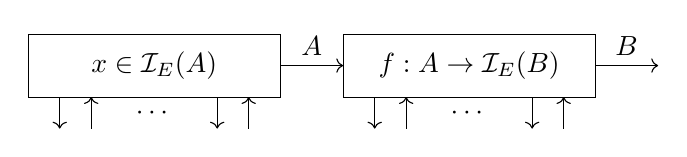
\begin{tikzpicture}[scale=0.4]
        \begin{scope}[xshift=-10cm]
          \draw (-4,-1) rectangle (4,1);
          \node (x) at (0,0) {$x \in \mathcal{I}_E(A)$};
          \draw[->] (-3, -1) -- (-3, -2);
          \draw[->] (-2, -2) -- (-2, -1);
          \node[below] at (0, -1) {$\cdots$};
          \draw[->] (2, -1) -- (2, -2);
          \draw[->] (3, -2) -- (3, -1);
        \end{scope}
        \draw[->] (-6,0) -- node[above] {$A$} (-4,0);
        \begin{scope}
          \draw (-4,-1) rectangle (4,1);
          \draw[->] (4,0) -- node[above] {$B$} (6,0);
          \node (f) at (0,0) {$f : A \rightarrow \mathcal{I}_E(B)$};
          \draw[->] (-3, -1) -- (-3, -2);
          \draw[->] (-2, -2) -- (-2, -1);
          \node[below] at (0, -1) {$\cdots$};
          \draw[->] (2, -1) -- (2, -2);
          \draw[->] (3, -2) -- (3, -1);
        \end{scope}
      \end{tikzpicture}
    }
    \only<2->{
      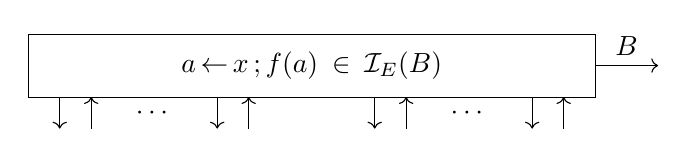
\begin{tikzpicture}[scale=0.4]
        \draw (-14,-1) rectangle (4,1);
        \node (xf) at (-5,0)
          {$a \mathop{\leftarrow} x \mathop{;} f(a) \: \in \: \mathcal{I}_E(B)$};
        \begin{scope}[xshift=-10cm]
          \draw[->] (-3, -1) -- (-3, -2);
          \draw[->] (-2, -2) -- (-2, -1);
          \node[below] at (0, -1) {$\cdots$};
          \draw[->] (2, -1) -- (2, -2);
          \draw[->] (3, -2) -- (3, -1);
        \end{scope}
        \begin{scope}
          \draw[->] (4,0) -- node[above] {$B$} (6,0);
          \draw[->] (-3, -1) -- (-3, -2);
          \draw[->] (-2, -2) -- (-2, -1);
          \node[below] at (0, -1) {$\cdots$};
          \draw[->] (2, -1) -- (2, -2);
          \draw[->] (3, -2) -- (3, -1);
        \end{scope}
      \end{tikzpicture}
    }
  \]
  \onslide<3->%
  \vspace{-1em}
  \[
    %\begin{tikzpicture}[scale=0.4]
    %  \draw (-2,-1) rectangle (2,1);
    %  \draw[->] (2,0) -- node[above] {$v \in A$} (5,0);
    %  \node (L) at (0,0) {$\mu_E^A(v)$};
    %\end{tikzpicture}
    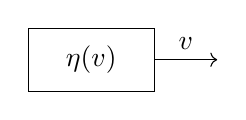
\begin{tikzpicture}[scale=0.4,baseline=0]
      \draw (-2,-1) rectangle (2,1);
      \draw[->] (2,0) -- node[above] {$v$} (4,0);
      \node (L) at (0,0) {$\eta(v)$};
    \end{tikzpicture}
    \qquad
    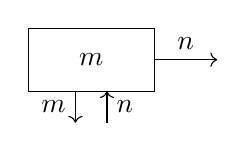
\begin{tikzpicture}[scale=0.4,baseline=0]
      %\small
      \draw (-2,-1) rectangle (2,1);
      \draw[->] (2,0) -- node[above] {$n$} (4,0);
      \node (L) at (0,0) {$m$};
      \draw[->] (-0.5, -1) -- node[left]  {$m$} (-0.5, -2);
      \draw[->] ( 0.5, -2) -- node[right] {$n$} ( 0.5, -1);
    \end{tikzpicture}
  \]
\end{block}

\onslide<4->
\begin{example}[Dequeuing from an array]
  \[
    \kw{deq} :=
      i \leftarrow \kw{inc}_1 \mathrel{;} \kw{get}[i]
  \]
  \[
    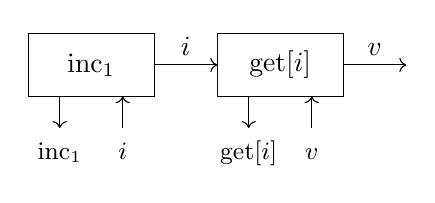
\begin{tikzpicture}[scale=0.4]
      \begin{scope}[xshift=-6cm]
        \draw (-2,-1) rectangle (2,1);
        \node (L) at (0,0) {$\kw{inc}_1$};
        \draw[->] (-1, -1) -- (-1, -2);
        \node[anchor=base] at (-1,-3) {\small $\kw{inc_1}$};
        \draw[->] (1, -2) -- (1, -1);
        \node[anchor=base] at (1,-3) {\small $i$};
        \draw[->] (2,0) -- node[above] {$i$} (4,0);
      \end{scope}
      \begin{scope}
        \draw (-2,-1) rectangle (2,1);
        \node (L) at (0,0) {$\kw{get}[i]$};
        \draw[->] (-1, -1) -- (-1, -2);
        \node[anchor=base] at (-1, -3) {\small $\kw{get}[i]$};
        \draw[->] (1, -2) -- (1, -1);
        \node[anchor=base] at (1, -3) {\small $v$};
        \draw[->] (2,0) -- node[above] {$v$} (4,0);
      \end{scope}
    \end{tikzpicture}%
  \]
\end{example}
\end{frame}
%}}}

\begin{frame}{Two-sided strategies} %{{{
  \begin{definition}
    A morphism $f : E \Rightarrow F$ is a family:
    \[
      f \in \prod_{(q : R) \in F} \mathcal{I}_E(R)
    \]
    \[
      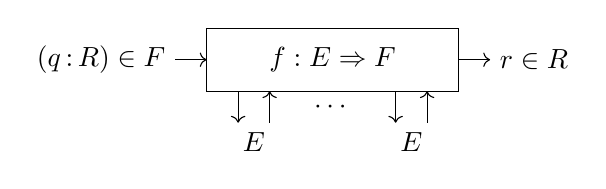
\begin{tikzpicture}[scale=0.4]
        \draw[->] (-5,0) node[left] {$(q \mathop{:} R) \in F$} -- (-4,0);
        \draw (-4,-1) rectangle (4,1);
        \draw[->] (4,0) -- (5,0) node[right] {$r \in R$};
        \node (f) at (0,0) {$f : E \Rightarrow F$};
        \draw[->] (-3, -1) -- (-3, -2);
        \draw[->] (-2, -2) -- (-2, -1);
        \node[below] at (0, -1) {$\cdots$};
        \draw[->] (2, -1) -- (2, -2);
        \draw[->] (3, -2) -- (3, -1);
        \node[below] at (-2.5, -2) {$E$};
        \node[below] at ( 2.5, -2) {$E$};
      \end{tikzpicture}
      \qquad
    \]
  \end{definition}
  \pause
  \begin{example}[Queue implementation]
    The morphism $M_\kw{q} : E_\kw{a} \Rightarrow E_\kw{q}$ is defined by:
    \[
      \begin{array}{l@{}l}
        \kw{enq}[v] & {} :=
          i \leftarrow \kw{inc}_2 \mathop{;} \kw{set}[i, v] \\
        \kw{deq} & {} :=
          i \leftarrow \kw{inc}_1 \mathop{;} \kw{get}[i]
      \end{array}
    \]
  \end{example}
\end{frame}
%}}}

\begin{frame}{Composition} %{{{
  \begin{block}{Substitution}
    The substitution $x[f]$ has the shape:
    \[
    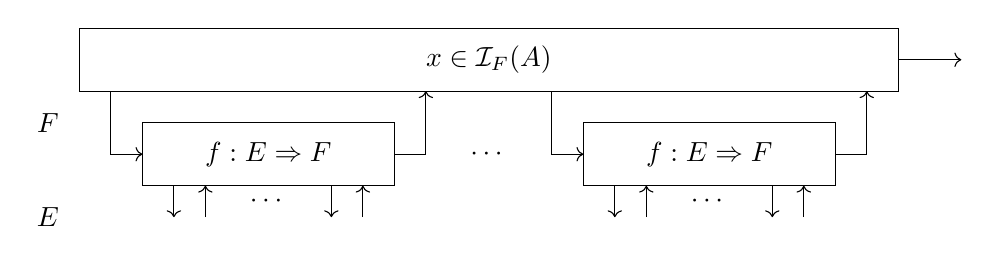
\begin{tikzpicture}[scale=0.4]
      \draw[->] (13, 3) -- (15, 3);
      \draw (-13, 2) rectangle (13, 4);
      \node at (0, 3) {$x \in \mathcal{I}_F(A)$};
      \begin{scope}[xshift=-7cm]
        \draw (-4,-1) rectangle (4,1);
        \draw[->] (-5, 2) |- (-4,0);
        \draw[->] (4,0) -| (5,2);
        \node (f) at (0,0) {$f : E \Rightarrow F$};
        \draw[->] (-3, -1) -- (-3, -2);
        \draw[->] (-2, -2) -- (-2, -1);
        \node[below] at (0, -1) {$\cdots$};
        \draw[->] (2, -1) -- (2, -2);
        \draw[->] (3, -2) -- (3, -1);
      \end{scope}
      \node at (0, 0) {$\cdots$};
      \begin{scope}[xshift=7cm]
        \draw (-4,-1) rectangle (4,1);
        \draw[->] (-5, 2) |- (-4,0);
        \draw[->] (4,0) -| (5,2);
        \node (f) at (0,0) {$f : E \Rightarrow F$};
        \draw[->] (-3, -1) -- (-3, -2);
        \draw[->] (-2, -2) -- (-2, -1);
        \node[below] at (0, -1) {$\cdots$};
        \draw[->] (2, -1) -- (2, -2);
        \draw[->] (3, -2) -- (3, -1);
      \end{scope}
      \node at (-14,  1) {$F$};
      \node at (-14, -2) {$E$};
    \end{tikzpicture}
    \]
    It can be used to define composition of morphisms.
  \end{block}
  \pause
  \begin{example}[Queue rotation]
    \vspace{-1em}
    \[ \begin{array}{r@{{} \in {}}c@{\quad := \quad}l}
      \kw{rot} & \mathcal{I}_{E_\kw{q}}(\mathbbm{1}) &
        v \mathop{\leftarrow} \kw{deq} \mathop{;} \kw{enq}[v] \\
      \kw{rot}[M_\kw{q}] & \mathcal{I}_{E_\kw{a}}(\mathbbm{1}) &
        i \mathop{\leftarrow} \kw{inc}_1 \mathop{;}
        v \mathop{\leftarrow} \kw{get}[i] \mathop{;}
        j \mathop{\leftarrow} \kw{inc}_2 \mathop{;}
        \kw{set}[j, v]
    \end{array} \]
  \end{example}
\end{frame}
%}}}

\begin{frame}{State} %{{{
  \begin{definition}[Extending a signature with state]
    We can annotate all calls and returns in $E$ with a state $k \in S$:
    \[
      E@S :=
        \{ m@k : N \times S \mid
           m {:} N \in E, k \in S \}
    \]
  \end{definition}
  \pause
  \only<1-2>{
  \begin{example}[Queue layer interface]
    {}
    \[
      S_\kw{q} := V^* \qquad
      L_\kw{q} : \varnothing \Rightarrow E_\kw{q}@S_\kw{q}
    \]
    \vspace{-1em}
    \[\begin{array}{r@{\:}l}
      \kw{enq}[v]@\vec{q} &:= \eta(*@\vec{q}v) \\
      \kw{deq}@\vec{q} &:=
        \bigsqcup_{v \! \vec{p} = \vec{q}} \eta(v@\vec{p})
    \end{array}\]
    {}
    \[
      \kw{rot}@S_\kw{q} :
        S_\kw{q} \rightarrow
        \mathcal{I}_{E_\kw{q}@S_\kw{q}}(\mathbbm{1} \times S_\kw{q})
    \] \[
      \kw{rot}@S_\kw{q}[L_\kw{q}] :
        S_\kw{q} \rightarrow
        \mathcal{I}_\varnothing(\mathbbm{1} \times S_\kw{q})
      \vspace{1ex}
    \]
  \end{example}
  }
  \only<3>{
  \begin{example}[Array layer interface]
    \[
      S_\kw{a} := V^\mathbb{N} \times \mathbb{N} \times \mathbb{N}
      \qquad
      L_\kw{a} : \varnothing \Rightarrow E_\kw{a}@S_\kw{a}
    \]
    \vspace{-1em}
    \[\begin{array}{r@{\:}l}
      \kw{get}[i]@(t, c_1, c_2) &:= \eta(t_i@(t, c_1, c_2))
      \\
      \kw{set}[i, v]@(t, c_1, c_2) &:= \eta(*@(t[i \leftarrow v], c_1, c_2))
      \\
      \kw{inc}_1@(t, c_1, c_2) &:= \eta(c_1@(t, c_1 + 1, c_2))
      \\
      \kw{inc}_2@(t, c_1, c_2) &:= \eta(c_2@(t, c_1, c_2 + 1))
    \end{array}\]
    {}
    \[
      M_\kw{q}@S_\kw{a} :
        E_\kw{a}@S_\kw{a} \Rightarrow E_\kw{q}@S_\kw{a}
      \qquad
      M_\kw{q}@S_\kw{a} \circ L_\kw{a} :
        \varnothing \Rightarrow E_\kw{q}@S_\kw{a}
    \]
  \end{example}
  }
\end{frame}
%}}}

\begin{frame}{Data abstraction} %{{{
  \begin{definition}
    A simulation relation $R \subseteq S_2 \times S_1$
    can be encoded as a morphism:
    \[
      \begin{array}{ccc}
        %L_2 : \varnothing \Rightarrow E@S_2 & &
        %L_1 : \varnothing \Rightarrow E@S_1 \\[1ex]
        R^*_E : E@S_2 \Rightarrow E@S_1 & &
        R_*^E : E@S_1 \Rightarrow E@S_2 \\[1ex]
        R^*_E \circ L_2 \sqsubseteq L_1 &
        \Leftrightarrow &
        L_2 \sqsubseteq R_*^E \circ L_1
      \end{array}
    \]
  \end{definition}
  \pause
  \begin{example}[Translating between array and queue states]
    \[
      \vec{q} \mathrel{R} (t, c_1, c_2)
      \quad \Leftrightarrow \quad
      c_1 \le c_2 \:\wedge\:
      \vec{q} = t_{c_1} \cdots t_{c_2 - 1}
    \]
    The layer interface
    $R^*_{E_q} \circ L_q : \varnothing \Rightarrow E_\kw{q}@S_\kw{a}$
    becomes:
    \begin{align*}
      \kw{enq}[v]@(t, c_1, c_2) &:=
        \bigsqcup_{\vec{q} = t_{c_1}\cdots t_{c_2}} \:
        \bigsqcap_{(t', c_1', c_2') | \vec{q}v = t'_{c_1'} \cdots t'_{c_2'}}
        \eta(*@(t', c_1', c_2')) \\
      \kw{deq}@(t, c_1, c_2) &:=
        \bigsqcup_{v\vec{q} = t_{c_1}\cdots t_{c_2}} \:
        \bigsqcap_{(t', c_1', c_2') | \vec{q} = t'_{c_1'} \cdots t'_{c_2'}}
        \eta(v@(t', c_1', c_2'))
    \end{align*}
  \end{example}
\end{frame}
%}}}

\begin{frame}[fragile]{Certified abstraction layers} %{{{
    \[
        L_\kw{a} \vdash M_\kw{q} : L_\kw{q}
        \qquad \qquad \quad \:\:
        R^*_{E_\kw{q}} \circ L_\kw{q} \sqsubseteq
          M_\kw{q}@S_\kw{a} \circ L_\kw{a}
        \quad
    \]
    \vspace{1em}
    \[
      \begin{prooftree}
        %\hypo{C}
        \infer0[$L_\kw{q}$]{
          \begin{array}{c}
            R \\
            \fbox{$\qquad M_\kw{q} \qquad$}
          \end{array}}
        \infer1[$L_\kw{a}$]{}
      \end{prooftree}
      \qquad \qquad
      \begin{tikzpicture}[xscale=2,yscale=1.5,baseline=0.66cm]
        \node (O) at (0,0) {$\varnothing$};
        \node (Lq) at (0,1) {$E_\kw{q}@S_\kw{q}$};
        \node (La) at (1,0) {$E_\kw{a}@S_\kw{a}$};
        \draw[->] (O) -- node[left] {\small $L_\kw{q}$} (Lq);
        \draw[->] (O) -- node[below] {\small $L_\kw{a}$} (La);
        \only<2->{
          \begin{scope}[overlay]
            \node (Eq) at (2,1) {$E_\kw{q}$};
            \node (Ea) at (2,0) {$E_\kw{a}$};
            \draw[->] (Ea) -- node[right] {\small $M_\kw{q}$} (Eq);
          \end{scope}
        }
        \only<3->{
          \node (Lqa) at (1,1) {$E_\kw{q}@S_\kw{a}$};
          \draw[->,dashed,overlay] (La) -- node[right]
            {\small $M_\kw{q}@S_\kw{a}$} (Lqa);
        }
        \only<4->{
          \draw[->,overlay] (Lq) -- node[above] {\small $R^*_{E_\kw{q}}$} (Lqa);
        }
        \only<5->{
          \node at (0.5,0.5) {$\sqsubseteq$};
        }
      \end{tikzpicture}
      \qquad
    \]
\end{frame}
%}}}

%}}}

\section{CompCertO} %{{{

\begin{frame}{Semantic model}
\end{frame}

\begin{frame}{Simulations}
\end{frame}

\begin{frame}{Vertical composition}
  \centering
  $\begin{array}{c}
    \kw{id} : A \Leftrightarrow A
    \qquad
    L \le_{\kw{id} \twoheadrightarrow \kw{id}} L
    \\[2em]
    {\begin{prooftree}
      \hypo{\mathbb{R} : A_1 \Leftrightarrow A_2}
      \hypo{\mathbb{S} : A_2 \Leftrightarrow A_3}
      \infer2{\mathbb{R} \cdot \mathbb{S} : A_1 \Leftrightarrow A_3}
    \end{prooftree}}
    \\[2em]
    {\begin{prooftree}
      \hypo{L_1 \le_{\mathbb{R}_A \twoheadrightarrow \mathbb{R}_B} L_2}
      \hypo{L_2 \le_{\mathbb{S}_A \twoheadrightarrow \mathbb{S}_B} L_3}
      \infer2{
        L_1 \le_{\mathbb{R}_A \cdot \mathbb{S}_A \twoheadrightarrow
                 \mathbb{R}_B \cdot \mathbb{S}_B} L_3}
    \end{prooftree}}
  \end{array}
  \qquad
  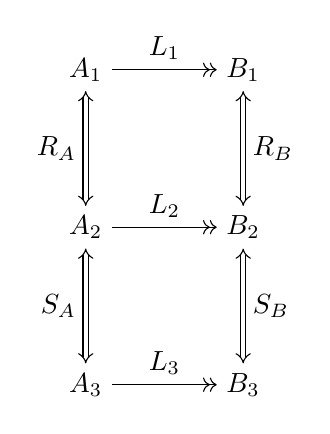
\begin{tikzpicture}[baseline,scale=1]
    \node (A1) at (-1,  2) {$A_1$};
    \node (A2) at (-1,  0) {$A_2$};
    \node (A3) at (-1, -2) {$A_3$};
    \node (B1) at ( 1,  2) {$B_1$};
    \node (B2) at ( 1,  0) {$B_2$};
    \node (B3) at ( 1, -2) {$B_3$};
    \draw (A1) edge[->>] node[auto] {$L_1$} (B1);
    \draw (A2) edge[->>] node[auto] {$L_2$} (B2);
    \draw (A3) edge[->>] node[auto] {$L_3$} (B3);
    \begin{scope}[double equal sign distance, {Implies[]}-{Implies[]}]
      \draw (A1) edge[double] node[auto,swap] {$\mathbb{R}_A$} (A2);
      \draw (B1) edge[double] node[auto] {$\mathbb{R}_B$} (B2);
      \draw (A2) edge[double] node[auto,swap] {$\mathbb{S}_A$} (A3);
      \draw (B2) edge[double] node[auto] {$\mathbb{S}_B$} (B3);
    \end{scope}
  \end{tikzpicture}
  $
\end{frame}

\begin{frame}{Horizontal composition}
\end{frame}

\begin{frame}{Compilation passes}
  \tiny
  \centering
  \begin{tabular}{l r @{$\: \twoheadrightarrow \:$} l r @{\ } r}
    \hline
    Language/Pass & Outgoing & Incoming & \multicolumn{2}{c}{SLOC}
      \\
    \hline
    \textbf{Clight} & $\mathcal{C}$ & $\mathcal{C}$ & +17 & (+3\%) \\
    \emph{Thm.~\ref{thm:cklr-props}} &
      $(\kw{ext} + \kw{injp})^*$ &
      $(\kw{ext} + \kw{injp})^*$ &
      & \\
    \kw{SimplLocals} & $\kw{injp}$ & $\kw{inj}$ & -4 & (-1\%) \\
    \kw{Cshmgen} & \kw{id} & \kw{id} & +0 & (+0\%) \\
    \hline
    \textbf{Csharpminor} & $\mathcal{C}$ & $\mathcal{C}$ & +15 & (+4\%) \\
    \kw{Cminorgen} & $\kw{injp}$ & $\kw{inj}$ & -21 & (-2\%) \\
    \hline
    \textbf{Cminor} & $\mathcal{C}$ & $\mathcal{C}$ & +27 & (+3\%) \\
    \kw{Selection} & $\kw{wt} \cdot \kw{ext}$ & $\kw{wt} \cdot \kw{ext}$ &
      +43 & (+0\%) \\
    \hline
    \textbf{CminorSel} & $\mathcal{C}$ & $\mathcal{C}$ & +15 & (+3\%) \\
    \kw{RTLgen} & $\kw{ext}$ & $\kw{ext}$ & +8 & (+0\%) \\
    \hline
    \textbf{RTL} & $\mathcal{C}$ & $\mathcal{C}$ & +11 & (+2\%) \\
    $\kw{Tailcall}^\dagger$ & $\kw{ext}$ & $\kw{ext}$ & -1 & (-1\%) \\
    \kw{Inlining} & $\kw{injp}$ & $\kw{inj}$ & +58 & (+3\%) \\
    \kw{Renumber} & $\kw{id}$ & $\kw{id}$ & -14 & (-7\%) \\
    \emph{Thm.~\ref{thm:cklr-props}} &
      $\kw{inj}$ &
      $\kw{inj}$ &
      & \\
    $\kw{Constprop}^\dagger$ &
      $\kw{va} \cdot \kw{ext}$ & $\kw{va} \cdot \kw{ext}$ &
      -17 & (-2\%) \\
    $\kw{CSE}^\dagger$ &
      $\kw{va} \cdot \kw{ext}$ & $\kw{va} \cdot \kw{ext}$ &
      +3 & (+0\%) \\
    $\kw{Deadcode}^\dagger$ &
      $\kw{va} \cdot \kw{ext}$ & $\kw{va} \cdot \kw{ext}$ &
      -7 & (-1\%) \\
    %\st{Unusedglob} \\
    \kw{Allocation} &
      $\kw{wt} \cdot \kw{alloc}$ & $\kw{wt} \cdot \kw{alloc}$ &
      +13 & (+0\%) \\
    \hline
    \textbf{LTL} & $\mathcal{L}$ & $\mathcal{L}$ & +15 & (+6\%) \\
    \kw{Tunneling} & $\kw{ext}$ & $\kw{ext}$ & +2 & (+0\%) \\
    \kw{Linearize} & \kw{id} & \kw{id} & -15 & (-3\%) \\
    \hline
    \textbf{Linear} & $\mathcal{L}$ & $\mathcal{L}$ & +16 & (+7\%) \\
    \kw{CleanupLabels} & \kw{id} & \kw{id} & -10 & (-4\%) \\
    \kw{Debugvar} & \kw{id} & \kw{id} & -12 & (-3\%) \\
    \kw{Stacking} & \kw{stacking} & \kw{stacking} & +291 & (+11\%) \\
    \hline
    \textbf{Mach} & $\mathcal{M}$ & $\mathcal{M}$ & +100 & (+26\%) \\
    \kw{Asmgen} & \kw{asmgen} & \kw{asmgen} & +179 & (+6\%) \\
    \hline
    \textbf{Asm} & $\mathcal{A}$ & $\mathcal{A}$ & +53 & (+5\%) \\
    \hline
    \multicolumn{3}{r}{Total:} & +765 & (+2\%)
  \end{tabular}
\end{frame}

%}}}

\section{Conclusion} %{{{

\begin{frame}{Conclusion}
  Game semantics and dual nondeterminism go hand-in-hand:
  \begin{itemize}
    \item Angelic nondeterminism is already present in strategies
    \item Unrestricted dual nondeterminism completes the symmetry
  \end{itemize}

  Refinement-based game introduces several innovations:
  \begin{itemize}
    \item Combine game semantics and the refinement calculus
    \item Nondeterminism decoupled from the structure of plays
    \item Supports heterogenous components and data abstraction
  \end{itemize}
\end{frame}

%}}}

\begin{frame}{}
  \begin{center}
    Thank you!
  \end{center}
\end{frame}

%}}}

%\appendix %{{{
%
%\begin{frame}{Specifications as nondeterministic programs} %{{{
%  Angelic and demonic choice are powerful
%  \emph{specification} constructs.
%
%  \pause
%  In the context of specifications:
%  \begin{center}
%    \begin{tabular}{cc}
%      \hline
%      Angelic choice ($\sqcup$) & Demonic choice ($\sqcap$) \\
%      \hline
%      Must satisfy both & Can satisfy either \\
%      Stronger guarantees & Implementation freedom \\
%      Environment & System \\
%      Increases with $\sqsubseteq$ & Decreases with $\sqsubseteq$ \\
%      \hline
%    \end{tabular}
%  \end{center}
%\end{frame}
%%}}}
%
%\begin{frame}{Abstraction} %{{{
%To formulate correctness properties,
%we will encode simulation relations as morphisms:
%\[
%  %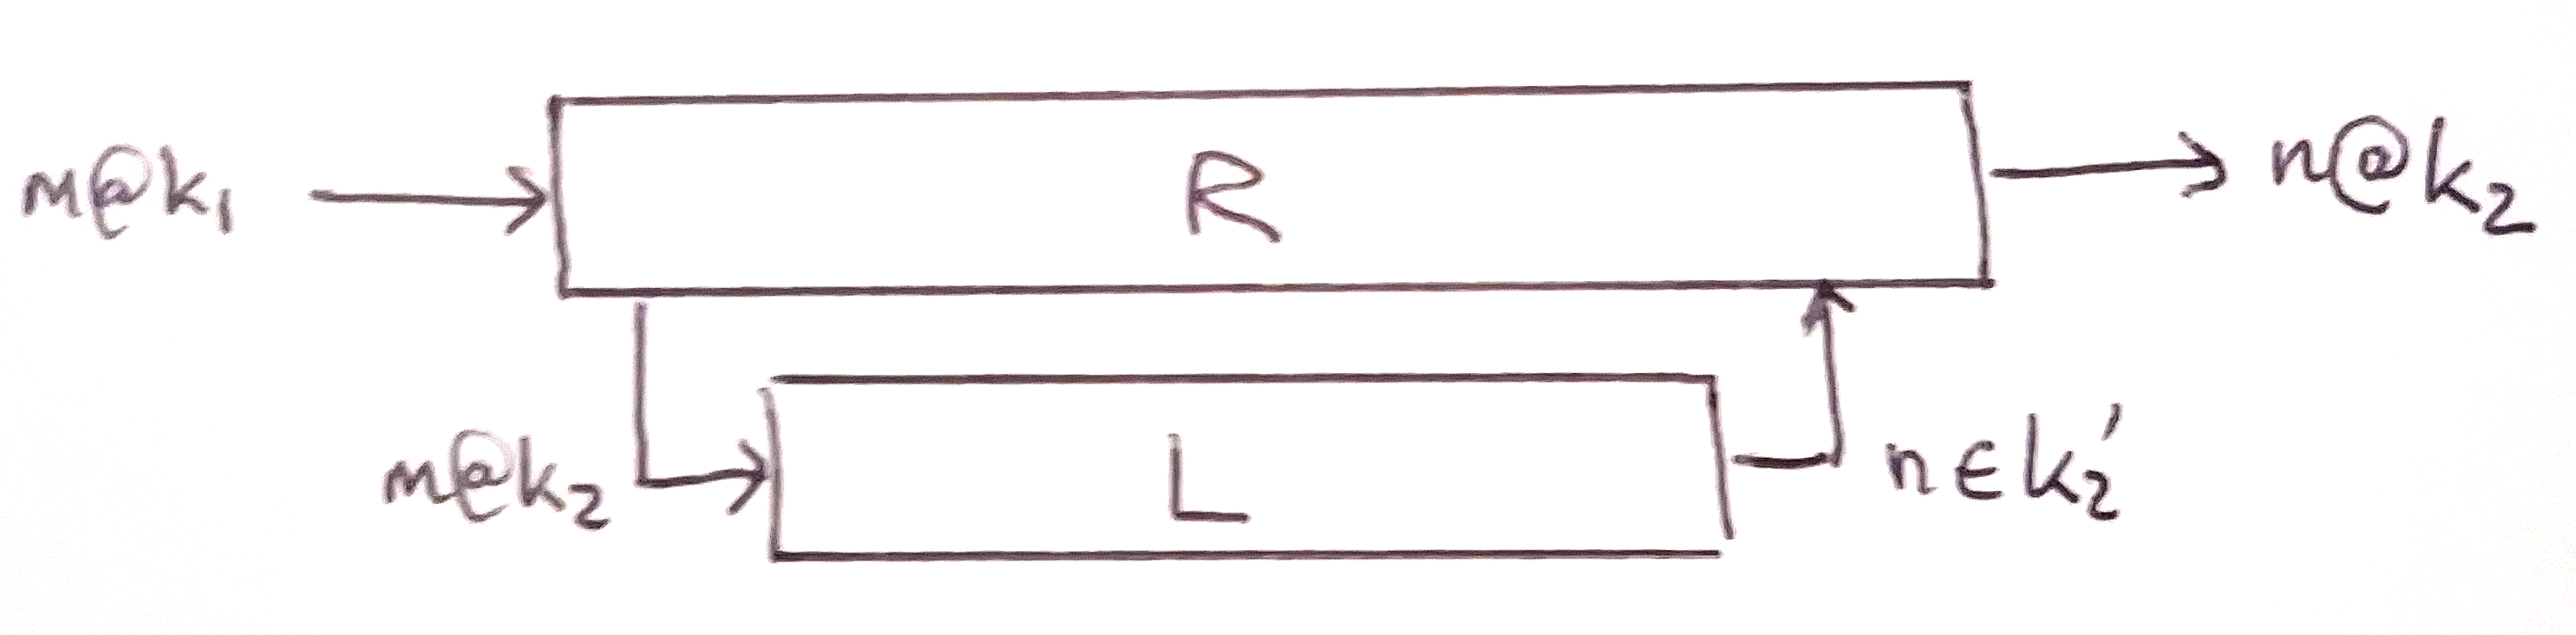
\includegraphics[scale=0.07]{simrel}
%\]
%and need to define an appropriate notion of refinement,
%so that layer correctness can be expressed as:
%\[
%  R^*_{E_2} \!\circ L_2 \: \sqsubseteq \: \llbracket M \rrbracket_{L_1}
%  \: \Leftrightarrow \:
%  L_1 \vdash_R M : L_2
%  \: \Leftrightarrow \:
%  L_2 \: \sqsubseteq \: R_*^{E_2} \!\circ \llbracket M \rrbracket_{L_1} \,.
%\]
%However,
%this requires a satisfactory treatment
%of \emph{dual nondeterminism} and
%\emph{alternating refinement}
%in the context of our game model.
%\end{frame}
%%}}}
%
%\section*{Introduction} %{{{
%
%\begin{frame}[fragile]{Why this gap?} %{{{
%  \centering
%  \begin{tabular}{cc}
%    \hline
%    Traditional focus &
%    What we need
%    \\
%    \hline
%    \\
%    \parbox{.45\textwidth}{
%      \centering
%      Precisely characterize \\ language features
%    } &
%    \parbox{.45\textwidth}{
%      \centering
%      General-purpose models \\ to embed anything
%    } \\[1.5em]
%    \parbox{.45\textwidth}{
%      \centering
%      Program equivalence, \\ full abstraction
%    } &
%    \parbox{.45\textwidth}{
%      \centering
%      Refinement and specifications
%    } \\[1.5em]
%    High-order computation &
%    Simple and mechanizable \pause \\[1.5em]
%    \hline
%  \end{tabular}
%
%  \emph{Bottom line:}
%  There is a lot of theory to draw from,
%  but current research focus
%  makes it hard to use in the context of verification.
%\end{frame}
%
%\begin{frame}{Generality}
%  Precedents for compositional certified systems:
%  \begin{itemize}
%    \item CompCert passes and languages
%    \item Certified abstraction layers (CertiKOS)
%    \item In both cases, \emph{uniformity} is key
%  \end{itemize}
%
%  Challenges for going further:
%  \begin{itemize}
%    \item Broad variety of models and techniques
%    \item 
%  \end{itemize}
%  The variety of models and techniques used
%  by existing 
%\end{frame}
%
%\begin{frame}{Refinement and nondeterminism}
%  Refinement:
%  \begin{itemize}
%    \item Uniform treatment of programs and specifications
%  \end{itemize}
%
%  Nondeterminism:
%  \begin{itemize}
%    \item Specifications allowing range of behaviors
%    \item Behavior outside of the system's control
%  \end{itemize}
%\end{frame}
%
%
%\begin{frame}{Contributions}
%  We introduce models which:
%  \begin{itemize}
%    \item Incorportate nondeterminism and refinement
%    \item Are general enough to embed various verif.
%    \item 
%  \end{itemize}
%\end{frame}
%
%%}}}
%
%%
%%\begin{frame}{Challenge} %{{{
%%  \begin{center}
%%    Goal: to build large-scale certified systems
%%  \end{center}
%%
%%  Certified system:
%%  accompanied by a formal specification
%%  and proof of correctness.
%%
%%  State of the art:
%%  we can build certified system components
%%  of significant size.
%%
%%  Next step:
%%  can we compose certified components
%%  to obtain large-scale certified systems?
%%\end{frame}
%%%}}}
%%
%%\begin{frame}{The DeepSpec project} %{{{
%%  DeepSpec is an NSF expedition project
%%  seeking to construct large-scale certified systems
%%  by connecting existing components
%%  certified in the Coq proof assistant.
%%
%%  Key idea:
%%  use specifications as \emph{interfaces}
%%
%%  Precedent:
%%  CompCert, CertiKOS
%%
%%  Limitation:
%%  rely on uniform semantic model
%%\end{frame}
%%%}}}
%%
%%\begin{frame}{CompCert} %{{{
%%  CompCert is a certified compiler from C to assembly.
%%
%%  Final theorem:
%%  the behavior of the assembly program
%%  emitted by the compiler
%%  refines that of the C program.
%%
%%  Compositionality:
%%  \begin{itemize}
%%    \item A similar theorem is established for each \emph{pass}
%%    \item Semantics of intermediate languages serve as intermediate specifications
%%    \item Passes can be composed when the target language of one
%%      coincides with the source language of the next
%%  \end{itemize}
%%\end{frame}
%%%}}}
%%
%%\begin{frame}{Problem statement} %{{{
%%  Our goal is to enable the construction of large-scale,
%%  heterogeneous certified systems.
%%  \begin{itemize}
%%  \pause \item
%%    \emph{Certified software}
%%    comes with
%%    a formal specification and
%%    a mechanized proof of correctness.
%%    %Researchers have produced
%%    %certified compilers, OS kernels, file systems,
%%    %processor designs, etc.
%%  \pause \item
%%    To scale it up,
%%    we need general-purpose semantic models
%%    which can embed and link various \emph{certified components}.
%%  \pause \item
%%    We believe a synthesis of
%%    game semantics and stepwise refinement approaches
%%    can be up to the task.
%%  \pause \item
%%    This work is a first step in this direction.
%%  \end{itemize}
%%
%%We want to use them as \emph{certified components}
%%to build large-scale, end-to-end certified systems.
%%However the diversity of techniques and semantic models
%%used across projects makes this difficult.
%%
%%Therefore, our goal is to:
%%\begin{itemize}
%%  \item
%%    Build a hierarchy of general-purpose semantic models
%%    for certified system components;
%%  \item
%%    Embed the semantics, specifications and proofs of
%%    existing projects into common models
%%    where they could be connected.
%%\end{itemize}
%%\end{frame}
%%}}}
%%
%
%%}}}
%
%\section*{CertiKOS and Certified Abstraction Layers} %{{{
%
%\begin{frame}{Layer interfaces} %{{{
%  Each layer interface $L$ consists of:
%  \begin{itemize}
%    \item
%      A \emph{signature} $\Sigma$ describing its primitive operations;
%    \item
%      A set $S$ of \emph{abstract states};
%    \item
%      A \emph{specification} for each operation $\kw{op} \in \Sigma$.
%  \end{itemize}
%
%  The specification of
%  $\kw{op} : A_1 \times \cdots \times A_n \rightarrow B$,
%  is given as:
%  \[
%    L.\kw{op} :
%      A_1 \times \cdots \times A_n \rightarrow
%      S \rightarrow \mathcal{P}^1(B \times S)
%  \]
%  The result can be a singleton $\{v@s\}$
%  or $\varnothing$ (undefined).
%\end{frame}
%%}}}
%
%\begin{frame}{Example: overlay interface} %{{{
%  $L_\kw{bq}$ provides a queue with values in $V$ and capacity $N = 4$:
%  \[
%    %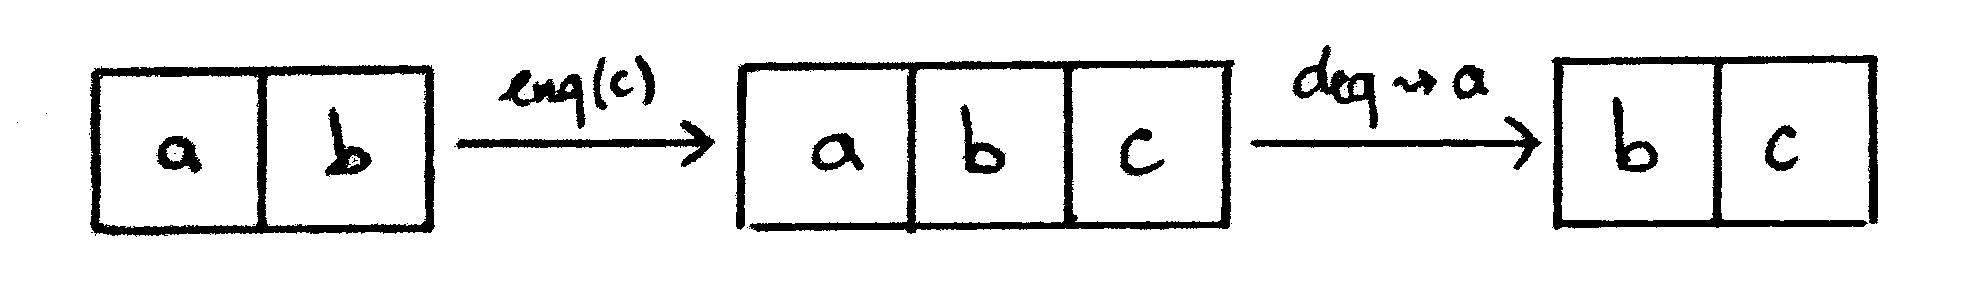
\includegraphics[scale=0.1]{enq_deq}
%  \]
%  The signature has two operations:
%  \begin{align*}
%    \kw{enq} &: V \rightarrow \mathbbm{1} \\
%    \kw{deq} &: \mathbbm{1} \rightarrow V
%  \end{align*}
%  The states are taken in $S_\kw{bq} := V^+$
%  and the specifications are:
%  \begin{align*}
%    L_\kw{bq}.\kw{enq}(v)@\vec{q} &:= \{ * @ \vec{q} v \mid |\vec{q}| < N \} \\
%    L_\kw{bq}.\kw{deq}(*)@\vec{q} &:= \{ v @ \vec{p} \: \mid \vec{q} = v \vec{p} \}
%  \end{align*}
%\end{frame}
%%}}}
%
%\begin{frame}{Client code} %{{{
%  Since specifications have the type:
%  \[
%    L.\kw{op} :
%      A_1 \times \cdots \times A_n \rightarrow
%      S \rightarrow \mathcal{P}^1(B \times S) \,,
%  \]
%  the monad $T(B) := S \rightarrow \mathcal{P}^1(B \times S)$
%  can be used to define sequential composition and
%  interpret client programs.
%
%  For example, using the free monad associated with $\Sigma_\kw{bq}$:
%  \[
%    \kw{rot} \in F_\kw{bq}(V) :=
%      v \leftarrow \kw{deq} \mathop{;}
%      \kw{enq}(v) \mathop{;}
%      \eta(v)
%  \]
%  This program can be evaluated on $L_\kw{bq}$ as:
%  \[
%    \llbracket \kw{rot} \rrbracket_{L_\kw{bq}} \in T_\kw{bq}(V) :=
%      v \leftarrow L_\kw{bq}.\kw{deq} \mathop{;}
%      L_\kw{bq}.\kw{enq}(v) \mathop{;}
%      \eta(v)
%  \]
%\end{frame}
%%}}}
%
%\begin{frame}{Layer implementation} %{{{
%  A layer implementation $L_1 \vdash M : L_2$
%  associates to each operation:
%  \[
%    \kw{op} : A_1 \times \cdots \times A_n \rightarrow B
%      \: \in \: \Sigma_2
%  \]
%  code which implements it in terms of $L_1$:
%  \[
%    M.\kw{op} : A_1 \times \cdots \times A_n \rightarrow F_1(B) \,.
%  \]
%
%  We can then write $\llbracket M \rrbracket_{L_1}$
%  to describes a layer interface obtained by
%  evaluating $M$
%  on top of the underlay interface $L_1$:
%  \[
%    \llbracket M \rrbracket_{L_1}.\kw{op} :=
%      \llbracket M.\kw{op} \rrbracket_{L_1}
%    \qquad (\kw{op} \in \Sigma_2)
%  \]
%\end{frame}
%%}}}
%
%\begin{frame}{Example: underlay interface} %{{{
%  Consider the underlay interface
%  $L_\kw{rb}$ provides a ring buffer with elements of $V$ and size $N = 4$:
%  \[
%    %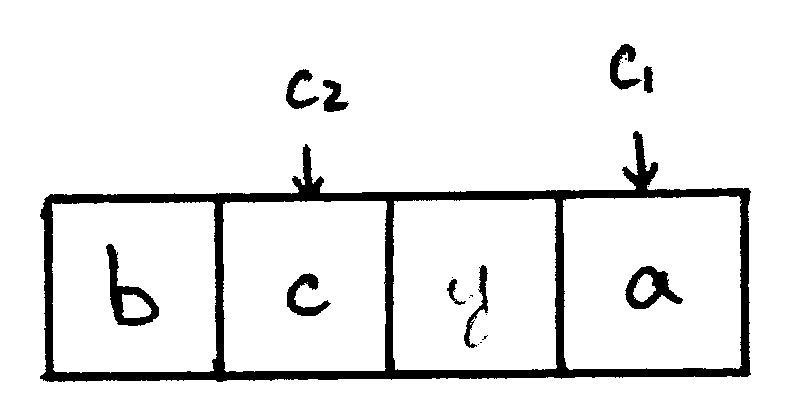
\includegraphics[scale=0.1]{ringbuf}
%  \]
%  States are taken in:
%  \[
%    S_\kw{rb} := V^N \times \mathbb{N} \times \mathbb{N}
%  \]
%  The operations are:
%  \begin{align*}
%    \kw{set} &: \mathbb{N} \times V \rightarrow \mathbbm{1} &
%    \kw{inc}_1 &: \mathbbm{1} \rightarrow \mathbb{N} \\
%    \kw{get} &: \mathbb{N} \rightarrow V &
%    \kw{inc}_2 &: \mathbbm{1} \rightarrow \mathbb{N}
%  \end{align*}
%\end{frame}
%%}}}
%
%\begin{frame}{Example: layer implementation} %{{{
%  Then a possible layer implementation of $L_\kw{bq}$
%  over $L_\kw{rb}$
%  is:
%  \begin{align*}
%    M_\kw{bq}.\kw{enq}(v) &:=
%      i \leftarrow \kw{inc}_2 \mathop{;} \kw{set}(i, v) \\
%    M_\kw{bq}.\kw{deq}(*) &:=
%      i \leftarrow \kw{inc}_1 \mathop{;} \kw{get}(i)
%  \end{align*}
%  Note that $\llbracket M_\kw{bq} \rrbracket_{L_\kw{rb}}$
%  inherits the states of $L_\kw{rb}$.
%  \begin{center}
%    %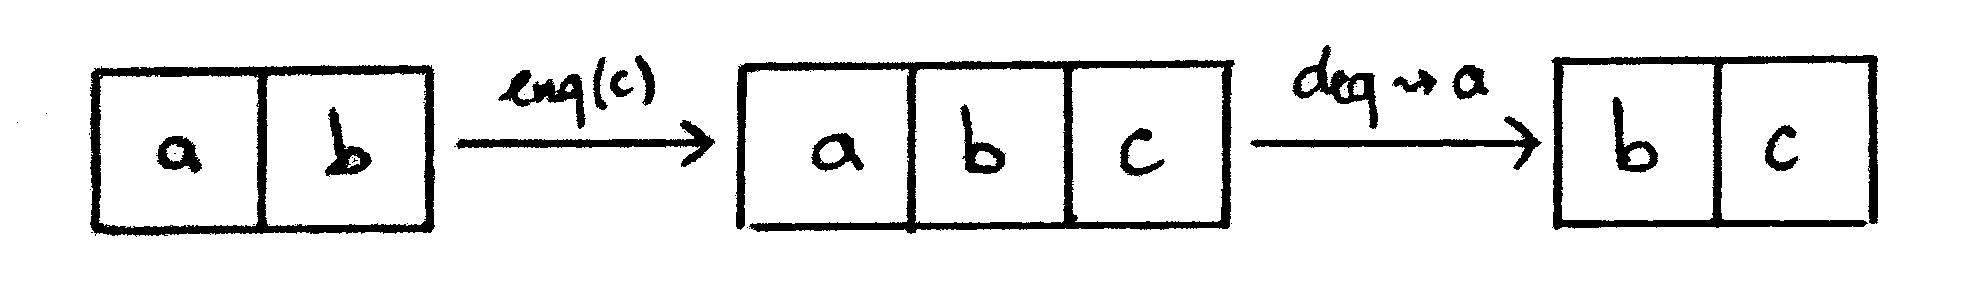
\includegraphics[scale=0.1]{enq_deq} \\
%    %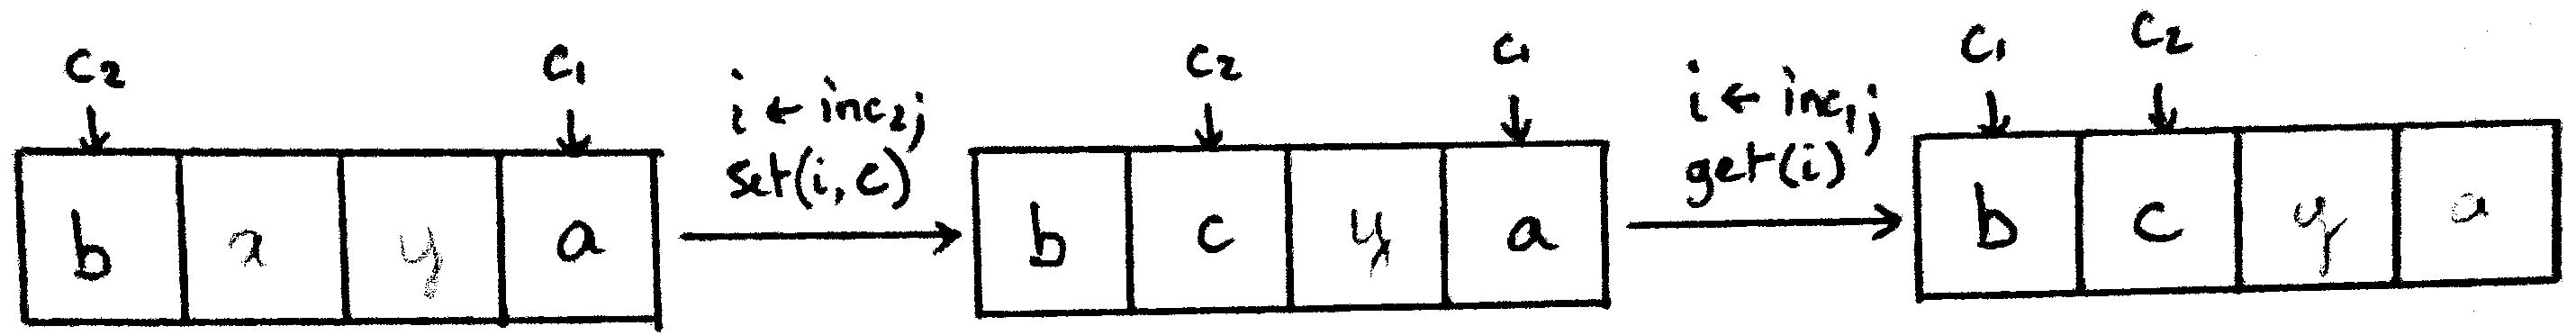
\includegraphics[scale=0.1]{ringbuf_enq_deq}
%  \end{center}
%\end{frame}
%%}}}
%
%\begin{frame}[fragile]{Layer correctness} %{{{
%  To establish the layer correctness property:
%  \[
%    \fbox{$L_1 \vdash M : L_2$}
%  \]
%  we need a \emph{simulation relation}
%  $R \subseteq S_2 \times S_1$ satisfying:
%  \[
%    \begin{tikzcd}[sep=large]
%      s_2 \ar[r, "L_2.\kw{op}"] \ar[d, "R"', dash] &
%      s_2' \ar[d, "R", dash, dashed] \\
%      s_1 \ar[r, "\llbracket M \rrbracket_{L_1}.\kw{op}"', dashed] &
%      s_1'
%    \end{tikzcd}
%  \]
%  The relation specifies how an overlay state $s_2$
%  may be realized as an underlay state $s_1$.
%\end{frame}
%%}}}
%
%%
%%\begin{frame}{Abstraction} %{{{
%%  Different layer interfaces use different kinds of abstract states,
%%  but $\llbracket M \rrbracket_L$ inherits its abstract states from $L$.
%%
%%  \pause
%%  So in truth we have:
%%  \[
%%    \begin{prooftree}
%%      \infer0[$L_2$]{\fbox{$\qquad M \qquad$}}
%%      \infer1[$L_1$]{}
%%    \end{prooftree}
%%    \qquad
%%    \begin{array}{c}
%%      \fbox{$L_1 \vdash_R M : L_2$} \\[1em]
%%      \forall C \: \bdot \:
%%      \llbracket C \rrbracket_{L_2} \sqsubseteq_R
%%      \llbracket C \oplus M \rrbracket_{L_1}
%%    \end{array}
%%  \]
%%
%%  \pause
%%  Simulation relations compose when we combine layers:
%%  \[
%%    \llbracket C \rrbracket_\kw{TSyscall}
%%    \sqsubseteq_{R_n \circ \cdots \circ R_1}
%%    \llbracket C \oplus M_n \oplus \cdots \oplus M_1 \rrbracket_\kw{MBoot}
%%  \]
%%\end{frame}
%%%}}}
%%
%%\begin{frame}{Example} %{{{
%%  \vspace{-2em}
%%  \[ L_\kw{rb} \vdash_R M_\kw{bq} : L_\kw{bq} \]
%%  \tiny
%%  \begin{align*}
%%    %
%%    % Overlay
%%    %
%%    & \fbox{$L_\kw{bq}$} &
%%      S_\kw{bq} &:= V^* \\
%%    \kw{enq} &: V \rightarrow \mathbbm{1} &
%%      L_\kw{bq}.\kw{enq}(v)@\vec{q} &:= \{ * @ \vec{q} v \mid |\vec{q}| < N \} \\
%%    \kw{deq} &: \mathbbm{1} \rightarrow V &
%%      L_\kw{bq}.\kw{deq}(*)@\vec{q} &:= \{ v @ \vec{p} \: \mid \vec{q} = v \vec{p} \}
%%    \\[1em]
%%    %
%%    % Implementation
%%    %
%%    & \fbox{$M_\kw{bq}$} &
%%      R &\subseteq S_\kw{bq} \times S_\kw{rb} \\
%%    M_\kw{bq}.\kw{enq}(v) &:= i \leftarrow \kw{inc}_2 ; \: \kw{set}(i, v) &
%%      \vec{q} \mathrel{R} (f, c_1, c_2) &\Leftrightarrow
%%      \: c_1 < N \:\wedge\: c_2 < N \:\wedge\: {}
%%    \\
%%    M_\kw{bq}.\kw{deq}(*) &:= i \leftarrow \kw{inc}_1 ; \: \kw{get}(i) &
%%      & \qquad \vec{q} = f_{c_1} \cdots f_{N-1} f_0 \cdots f_{c_2}
%%    \\[1em]
%%    %
%%    % Underlay
%%    %
%%    & \fbox{$L_\kw{rb}$} &
%%      S_\kw{rb} &:= V^N \times \mathbb{N} \times \mathbb{N}
%%    \\
%%    \kw{set} &: \mathbb{N} \times V \rightarrow \mathbbm{1} &
%%      L_\kw{rb}.\kw{set}(i, v)@(f, c_1, c_2) &:=
%%      \{ *@(f', c_1, c_2) \mid i < N \wedge f' = f[i := v] \}
%%    \\
%%    \kw{get} &: \mathbb{N} \rightarrow V &
%%      L_\kw{rb}.\kw{get}(i)@(f, c_1, c_2) &:=
%%      \{ f_i@(f, c_1, c_2) \mid i < N \}
%%    \\
%%    \kw{inc}_1 &: \mathbbm{1} \rightarrow \mathbb{N} &
%%      L_\kw{rb}.\kw{inc}_1@(f, c_1, c_2) &:=
%%      \{ c_1@(f, c_1', c_2) \mid
%%         c_1' = (c_1 + 1) \mathop{\mathrm{mod}} N \}
%%    \\
%%    \kw{inc}_2 &: \mathbbm{1} \rightarrow \mathbb{N} &
%%      L_\kw{rb}.\kw{inc}_2@(f, c_1, c_2) &:=
%%      \{ c_2@(f, c_1, c_2') \mid
%%         c_2' = (c_2 + 1) \mathop{\mathrm{mod}} N \}
%%  \end{align*}
%%\end{frame}
%%%}}}
%%
%%\begin{frame}{Limitations} %{{{
%%  As used in CertiKOS,
%%  certified abstraction layers have a number of limitations:
%%  \begin{itemize}
%%    \pause \item Fixed interaction model
%%    \pause \item Linking with CompCert is complicated
%%    \pause \item Horizontal composition is limited
%%    \pause \item We only consider \emph{closed} systems
%%  \end{itemize}
%%
%%  \pause
%%  To address them,
%%  we design a game semantics which can be used to embed:
%%  \begin{itemize}
%%    \pause \item Certified abstraction layers
%%    \pause \item Compositional module semantics for CompCert
%%    \pause \item Interaction trees
%%  \end{itemize}
%%\end{frame}
%%%}}}
%%
%
%%}}}
%
%\section*{Dual nondeterminism and refinement} %{{{
%
%\begin{frame}{Nondeterminism} %{{{
%  Nondeterminism occurs
%  when information is missing or forgotten:
%  \begin{itemize}
%    \item Inputs, environment behavior
%    \item Underspecified system, abstraction
%  \end{itemize}
%
%  In the context of games,
%  it is crucial to distinguish between
%  \emph{angelic} and \emph{demonic}
%  nondeterminism.
%  We will associate:
%  \begin{itemize}
%    \item \emph{angelic} nondeterminism
%      with choices of the environment;
%    \item \emph{demonic} nondeterminism
%      with choices of the system.
%  \end{itemize}
%\end{frame}
%%}}}
%
%\begin{frame}{Angelic nondeterminism} %{{{
%  Traditional strategies use angelic nondeterminism:
%  \begin{itemize}
%    \item a play corresponds to one possible interaction;
%    \item sets of plays range over environment choices.
%  \end{itemize}
%  Refinement corresponds to set inclusion ($\subseteq$).
%\end{frame}
%%}}}
%
%\begin{frame}{Angelic nondeterminism (example)} %{{{
%  Writing $\sqcup$ for angelic choices,
%  the negation function $x \mapsto - x$ on $\{-1, 0, 1\}$
%  can be expressed as:
%  \[
%    (-1 \mapsto 1) \sqcup (0 \mapsto 0) \sqcup (1 \mapsto -1)
%  \]
%
%  It satisfies the specifications:
%  \begin{align*}
%    (0 \mapsto 0) &\sqsubseteq
%      (-1 \mapsto 1) \sqcup (0 \mapsto 0) \sqcup (1 \mapsto -1) \\
%    (-1 \mapsto 1) \sqcup (1 \mapsto -1) &\sqsubseteq
%      (-1 \mapsto 1) \sqcup (0 \mapsto 0) \sqcup (1 \mapsto -1) \\
%    \bot &\sqsubseteq
%      (-1 \mapsto 1) \sqcup (0 \mapsto 0) \sqcup (1 \mapsto -1)
%  \end{align*}
%\end{frame}
%%}}}
%
%\begin{frame}{Demonic nondeterminism} %{{{
%  In verification,
%  we often want to express loose specifications:
%  \begin{itemize}
%    \item the specification allows a range of behaviors
%      from the system;
%    \item the implementation can choose one of them.
%  \end{itemize}
%  Refinement corresponds to set containement ($\supseteq$).
%\end{frame}
%%}}}
%
%\begin{frame}{Demonic nondeterminism (example)} %{{{
%  Writing $\sqcap$ for demonic choice,
%  the specification:
%  \[
%    (1 \mapsto 1) \sqcap (1 \mapsto -1)
%  \]
%  allows the system to map $1$ to either itself or its opposite.
%
%  Some possible refinements are:
%  \begin{align*}
%    (1 \mapsto 1) \sqcap (1 \mapsto -1) &\sqsubseteq
%      (x \mapsto x) \\
%    (1 \mapsto 1) \sqcap (1 \mapsto -1) &\sqsubseteq
%      (x \mapsto -x) \\
%    (1 \mapsto 1) \sqcap (1 \mapsto -1) &\sqsubseteq
%      (1 \mapsto -1)
%  \end{align*}
%\end{frame}
%%}}}
%
%\begin{frame}{Dual nondeterminism} %{{{
%  Certified abstraction layers use
%  both kinds of nondeterminism:
%  \[
%    %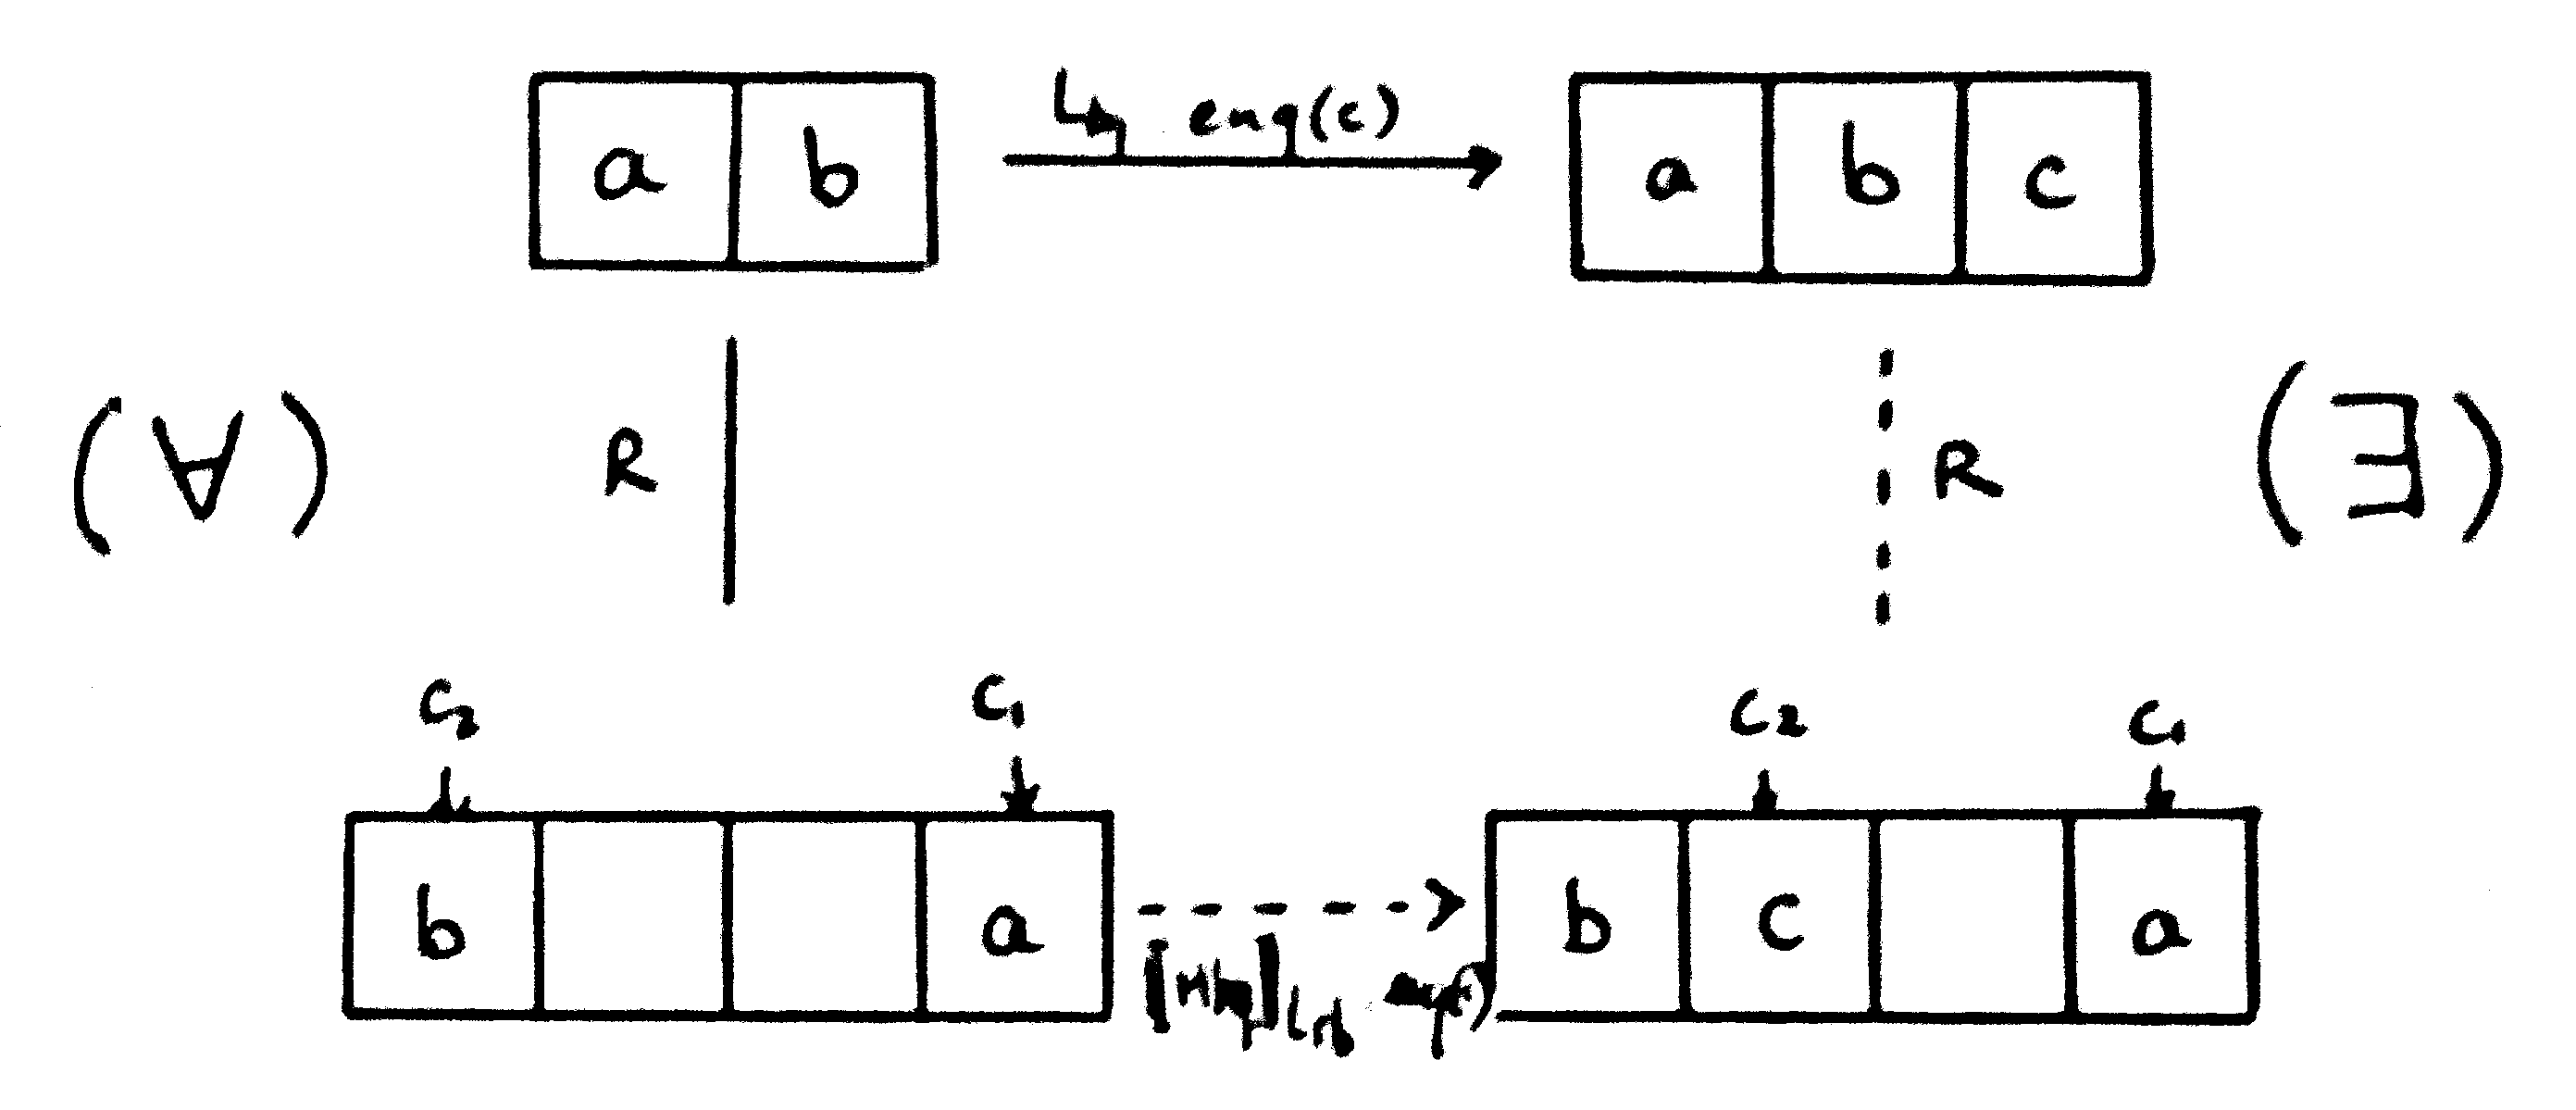
\includegraphics[scale=0.07]{layersim}
%  \]
%\end{frame}
%%}}}
%
%\begin{frame}{Strategy specifications} %{{{
%We use \emph{sets of sets} of plays
%to construct \emph{strategy specifications},
%equipped with a
%\emph{completely distributive lattice}
%structure:
%\begin{itemize}
%  \item Sups provide unbounded angelic choices
%  \item Infs provide unbounded demonic choices
%  \item Complete lattice: the model is insensitive to branching
%  \item Complete distributivity: angelic and demonic choices commute
%  \[
%      \bigsqcap_{i \in I} \bigsqcup_{j \in J_i} x_{i,j} =
%      \bigsqcup_{f \in (\prod_i J_i)} \bigsqcap_{i \in I} x_{i, f_i}
%  \]
%  \item $\bot$ is used to capture undesirable behaviors (only refines itself),
%    including silent divergence.
%\end{itemize}
%%Constructions are expected to be monotonic,
%%enabling congruent refinement.
%%Most preserve $\sqcup$ and $\sqcap$.
%\end{frame}
%%}}}
%
%\begin{frame}{Angelic nondeterminism and strategies} %{{{
%  Traditional strategies use
%  \emph{prefix-closed} sets of plays.
%  This is because plays \emph{already} have
%  a natural refinement ordering:
%  \[
%    m \sqsubseteq mn
%    \quad \mbox{ but } \quad
%    \{m\} \nsubseteq \{mn\}
%  \]
%  Using \emph{downsets}:
%  \[
%    {\downarrow} m = \{\epsilon, m\} \subseteq \{\epsilon, m, mn\} = {\downarrow} mn
%  \]
%
%  More generally,
%  downsets add arbitrary suprema to a poset:
%  \begin{itemize}
%    \item $(\mathcal{P}(A), {\subseteq})$ is the
%      free sup-lattice generated by the \emph{set} $A$
%    \item $(\mathcal{D}(A), {\subseteq})$ is the
%      free sup-lattice generated by the \emph{poset} $A$
%  \end{itemize}
%\end{frame}
%%}}}
%
%\begin{frame}{Demonic nondeterminism and strategy specifications} %{{{
%  Similarly,
%  using simple sets to add demonic nondeterminism to angelic strategies
%  doesn't work:
%  \[
%    \sigma \sqsubseteq \tau \nRightarrow
%    \{\sigma\} \nsupseteq \{\tau\}
%  \]
%  Using \emph{upsets}:
%  \[
%    \sigma \sqsubseteq \tau \Rightarrow
%    {\uparrow} \sigma \supseteq {\uparrow} \tau
%  \]
%
%  Upsets are dual to downsets:
%  \begin{itemize}
%    \item $(\mathcal{P}(A), {\supseteq})$ is the
%      free inf-lattice generated by the \emph{set} $A$
%    \item $(\mathcal{U}(A), {\supseteq})$ is the
%      free inf-lattice generated by the \emph{poset} $A$
%  \end{itemize}
%\end{frame}
%%}}}
%
%%
%%\begin{frame}{Refinement} %{{{
%%%\emph{Stepwise refinement} techniques
%%%treat programs, specifications and correctness
%%%in a uniform way.
%%%Specification constructs are added to the language,
%%%and the implementation is derived by
%%%incrementally replacing them
%%%by executable statements.
%%
%%In the context of Hoare logic and axiomatic semantics,
%%a~refinement $C_1 \sqsubseteq C_2$
%%means that any correctness property satisfied by $C_1$
%%will also be satisfied by $C_2$:
%%\[
%%    C_1 \sqsubseteq C_2 \: := \:
%%    \forall P Q \bdot
%%      \htr{P}{C_1}{Q} \Rightarrow
%%      \htr{P}{C_2}{Q}
%%\]
%%%Then the goal is to establish
%%%a sequence of refinements
%%%$C_1 \sqsubseteq \cdots \sqsubseteq C_n$
%%%to show that a program $C_n$ involving
%%%only executable constructions
%%%correctly implements a specification $C_1$.
%%
%%For games and open systems,
%%refinement is \emph{alternating}.
%%A refinement allows:
%%\begin{itemize}
%%  \item \emph{more} behaviors from the \emph{environment}
%%  \item \emph{fewer} behaviors form the system
%%\end{itemize}
%%\end{frame}
%%%}}}
%%
%%\begin{frame}[fragile]{Angelic and demonic choice} %{{{
%%The \emph{refinement calculus} 
%%is a framework for stepwise refinement
%%of imperative programs,
%%constructed around predicate transformer semantics,
%%featuring \emph{dual nondeterminism}:
%%\begin{itemize}
%%  \item \emph{Angelic choices} are resolved by an angel:
%%  \[
%%    \begin{prooftree}
%%      \hypo{\htr{P}{C_1}{Q}}
%%      \infer1{\htr{P}{C_1 \sqcup C_2}{Q}}
%%    \end{prooftree}
%%    \qquad
%%    \begin{prooftree}
%%      \hypo{\htr{P}{C_2}{Q}}
%%      \infer1{\htr{P}{C_1 \sqcup C_2}{Q}}
%%    \end{prooftree}
%%  \]
%%  \item \emph{Demonic choices} are resolved by a demon:
%%  \[
%%    \begin{prooftree}
%%      \hypo{\htr{P}{C_1}{Q}}
%%      \hypo{\htr{P}{C_2}{Q}}
%%      \infer2{\htr{P}{C_1 \sqcap C_2}{Q}}
%%    \end{prooftree}
%%  \]
%%\end{itemize}
%%Angelic and demonic choices correspond to meets and joins
%%with respect to the refinement ordering.
%%%Two fundamental operations
%%%to make it possible to express specifications.
%%%
%%%By giving lattice structure,
%%%we obtain a model insensivive to branching.
%%%Complete distributivity further allows
%%%angelic and demonic choices to commute:
%%\end{frame}
%%%}}}
%%
%%\begin{frame}{Strategies} %{{{
%%The traditional construction of strategies
%%uses \emph{angelic} nondeteminism
%%to range over the possible behaviors of the environment:
%%\[
%%  \mathcal{I}_E(A) := \mathcal{D}(\bar{P}_E(A))
%%\]
%%To enable demonic nondeterminism as well,
%%we will use the
%%\emph{free completely distributive lattice}
%%instead of downsets:
%%\[
%%  \mathcal{I}_E(A) := \mathbf{FCD}(\bar{P}_E(A))
%%\]
%%\end{frame}
%%%}}}
%%
%
%\begin{frame}[fragile]{Constructing strategy specifications} %{{{
%By combining the two,
%we obtain the
%the \emph{free completely distributive lattice} over a poset:
%\[
%  \mathbf{FCD}(A) := \mathcal{U}(\mathcal{D}(A))
%\]
%
%The inner layer corresponds to traditional angelic strategies,
%ranging over permissible behaviors of the environment.
%
%The outer layer adds demonic nondeterminism, \\
%ranging over permissible behaviors of the system.
%\end{frame}
%%}}}
%
%\begin{frame}[fragile]{Properties of $\mathbf{FCD}$} %{{{
%A more abstract description of $\mathbf{FCD}$
%is given by the adjunction:
%\[
%  \mathbf{FCD} : \mathbf{Pos} \rightleftarrows \mathbf{CDLat} : U
%  \qquad
%  \begin{tikzcd}
%    C \arrow[r, "\phi"] \arrow[rd, "f"'] &
%    \mathbf{FCD}(C) \arrow[d, "f^*_\phi", dashed] \\ & M
%  \end{tikzcd}
%\]
%Each element $x \in \mathbf{FCD}(C)$ can be written as:
%\[
%  x = \bigsqcap_{i \in I} \bigsqcup_{j \in J_i} \phi(c_{ij})
%  \qquad
%  f^*_\phi(x) = \bigsqcap_{i \in I} \bigsqcup_{j \in J_i} f(c_{ij})
%\]
%In other words,
%a complete homomorphism from $\mathbf{FCD}(C)$ into another lattice
%is completely determined by its image on $C$.
%\end{frame}
%%}}}
%
%\begin{frame}{Example: interaction primitives} %{{{
%For $m : N \in E$,
%we can use angelic nondeterminism to define
%the interaction primitive $\mathbf{I}_E^m \in \mathcal{I}_E(N)$
%as:
%\[
%  \mathbf{I}^m := \bigsqcup_{n \in N} \underline{m} n \underline{n}
%\]
%The family $\mathbf{I}_E : E \rightarrow E$
%also serves as the identity morphism,
%and can be depicted as:
%\[
%  %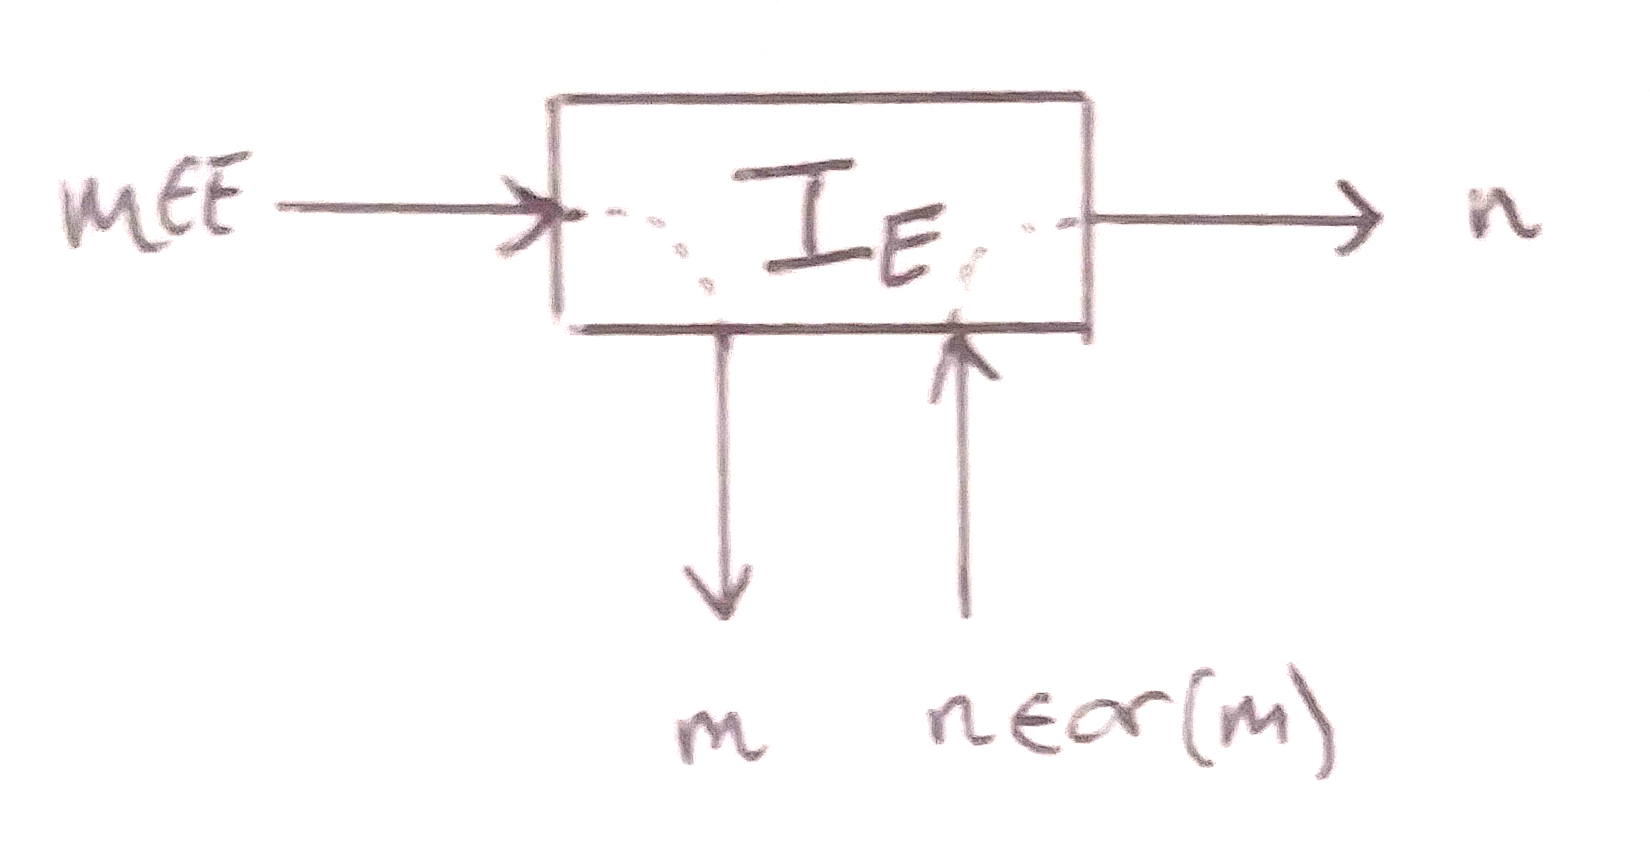
\includegraphics[scale=0.08]{int}
%\]
%\end{frame}
%%}}}
%
%\begin{frame}{Example: simulation relations} %{{{
%We use dual nondeterminism,
%to embed simulation relations as:
%\[
%  {\everymath={\displaystyle}
%  \begin{array}{r@{\:}c@{\:}c@{\:}c@{\:}l}
%  (R^*_E)^{m@k_1} := &
%    \bigsqcup_{k_2 \in R^{-1}(k_1)} &
%    n@k_2' \leftarrow \mathbf{I}^{m@k_2} ; &
%    \bigsqcap_{k_1' \in R(k_2')} &
%    \eta(n@k_1') \\[2.5em]
%  (R_*^E)^{m@k_2} := &
%    \bigsqcap_{k_1 \in R(k_2)} &
%    n@k_1' \leftarrow \mathbf{I}^{m@k_1} ; &
%    \bigsqcup_{k_2' \in R^{-1}(k_1')} &
%    \eta(n@k_2')
%  \end{array}}
%\]
%This establishes a Galois connexion
%which we can use to model abstraction.
%For $\sigma : 1 \rightarrow E@S_2$
%and $\tau : 1 \rightarrow E@S_1$,
%\[
%  R^*_{E_2} \!\circ \sigma \: \sqsubseteq \: \tau
%  \quad \Leftrightarrow \quad
%  \sigma \: \sqsubseteq \: R_*^{E_2} \!\circ \tau \,.
%\]
%\end{frame}
%%}}}
%
%%}}}
%
%\section*{Conclusion} %{{{
%
%\begin{frame}{Conclusion}
%\end{frame}
%
%%}}}
%
%%
%%\begin{frame}{Game semantics} %{{{
%%Game semantics is an approach to compositional semantics:
%%\begin{itemize}
%%  \item Types are interpreted as \emph{games}
%%    and terms as \emph{strategies}.
%%  \item Very general, lots of research to build on.
%%  \item Sometimes fairly complex.
%%\end{itemize}
%%
%%For our purposes:
%%\begin{itemize}
%%  \item Type structure helps us model heterogenous systems;
%%  \item First-order is good enough for system components,
%%    this simplifies things a lot;
%%  \item What about proofs?
%%\end{itemize}
%%\end{frame}
%%%}}}
%%
%%\section*{Effectful computations}
%%
%%\begin{frame}{Algebraic effects} %{{{
%%In the framework of \emph{algebraic effects}:
%%\begin{itemize}
%%  \item Terms represent computations;
%%  \item Operations represent effects;
%%  \item Arguments specify possible continuations.
%%\end{itemize}
%%
%%\begin{example}
%%The term
%%$\kw{readbit}(
%%  \kw{print}["\text{Hello}"](\kw{done}),
%%  \kw{print}["\text{World}"](\kw{done}))$
%%can~be read as a strategy:
%%\[
%%  \begin{tikzpicture}[scale=0.8]
%%    %\node (W) at (0,0) {};
%%    \node (R) at (0,-1) {$\kw{readbit}$};
%%    \node (W0) at (-2,-2) {$\kw{print}["\text{Hello}"]$};
%%    \node (W1) at (+2,-2) {$\kw{print}["\text{World}"]$};
%%    \node (K0) at (-2,-3) {$\kw{done}$};
%%    \node (K1) at (+2,-3) {$\kw{done}$};
%%    %\path (W) edge node[auto,swap] {$*$} (R);
%%    \path (R) edge node[auto,swap] {0} (W0);
%%    \path (R) edge node[auto] {1} (W1);
%%    \path (W0) edge node[auto,swap] {$*$} (K0);
%%    \path (W1) edge node[auto,swap] {$*$} (K1);
%%  \end{tikzpicture}
%%\]
%%\end{example}
%%\end{frame}
%%%}}}
%%
%%\begin{frame}{Plays}
%%\begin{definition}[Effect signature]
%%A set $E$ of operations
%%together with a mapping $\kw{ar} : E \rightarrow \mathbf{Set}$.
%%\end{definition}
%%
%%\begin{example}
%%\[
%%  E_\kw{io} :=
%%  \{ \kw{readbit} : \mathbbm{2}, \:
%%     \kw{print}[s] : \mathbbm{1}, \:
%%     \kw{done} : \varnothing \mid
%%     s \in \kw{string} \}
%%\]
%%\end{example}
%%
%%\begin{definition}[Plays for interactions]
%%The set $\bar{P}_E(A)$ is defined inductively by:
%%\[
%%  s \in \bar{P}_E(A) ::=
%%    \underline{v} \mid
%%    \underline{m} \mid
%%    \underline{m} n s
%%  \qquad
%%  (v \in A, m \in E, n \in \kw{ar}(m))
%%  \,,
%%\]
%%and ordered under prefix ($\underline{m} \sqsubseteq \underline{m} n s$).
%%\end{definition}
%%\end{frame}
%%
%%\begin{frame}[fragile]{Plays (drawing)}
%%  \[
%%  \begin{tikzpicture}[scale=0.5]
%%    \draw[->] (0,1) -| (1,0) node[below left] {$m_1$} -- (1,-2);
%%    \draw[->] (2,-2) -- (2,0) node[below right] {$n_1$};
%%    \draw[->] (2,0) -- (2,1) -| (6,0) node[below left] {$m_2$} -- (6,-2);
%%    {
%%    \tikzset{xshift=5cm}
%%    \draw[->] (2,-2) -- (2,0) node[below right] {$n_2$};
%%    \draw[->] (2,0) -- (2,1) -| (6,0) node[below left] {$m_3$} -- (6,-2);
%%    }
%%    \tikzset{xshift=5cm}
%%    \draw[->] (2,-2) -- (2,0) node[below right] {$n_1$};
%%
%%    \pmove{m_1} -- 
%%
%%  \end{tikzpicture}
%%  \]
%%\end{frame}
%
%%
%%
%%\begin{frame}{Interaction specifications}
%%The free completely distributive completion of
%%$\bar{P}_E$
%%gives us a version of the \emph{free monad}
%%on the effect signature $E$.
%%
%%\begin{definition}[Interaction specification monad]
%%\begin{itemize}
%%  \item $\mathcal{I}_E(A) := \mathbf{FCD}(\bar{P}_E(A))$.
%%  \item The unit $\eta^E_A : A \rightarrow \mathcal{I}_E(A)$
%%    is defined by $\eta^E_A(v) := \underline{v}$
%%  \item The extension of $f : A \rightarrow \mathcal{I}_E(B)$
%%    is defined by:
%%  \begin{align*}
%%    f^\dagger(\underline{v}) &:= f(v) \\
%%    f^\dagger(\underline{m}) &:= \underline{m} \\
%%    f^\dagger(\underline{m} n s) &:=
%%      \underline{m} \sqcup \underline{m} n f^\dagger(s)
%%  \end{align*}
%%\end{itemize}
%%\end{definition}
%%\end{frame}
%%
%%\begin{frame}{Summary}
%%An \emph{interaction specification} in $\mathcal{I}_E(A)$
%%triggers effects in $E$ and produces an outcome in $A$.
%%
%%$\mathcal{I}_E(A)$ is equipped with a completely distributive lattice
%%structure which models \emph{dual nondeterminism}.
%%\end{frame}
%%
%%\section*{Strategies}
%%
%%\begin{frame}{Interaction primitives and substitution}
%%A strategy specification $f : E \rightarrow F$
%%is a \emph{family} $(f^m)_{m \in F}$:
%%\[
%%     f^m \in \mathcal{I}_E(\kw{ar}(m)) \qquad
%%     (m \in F)
%%\]
%%The identity strategy $\mathbf{I} : E \rightarrow E$
%%is the family of \emph{interaction primitives}:
%%\[
%%  \mathbf{I}_E^m :=
%%    \bigsqcup_{n \in \kw{ar}(m)} \underline{m} n \underline{n}
%%\]
%%The composition of $f : E \rightarrow F$ and $g : F \rightarrow G$
%%will be defined as:
%%\[
%%    (g \circ f)^m := g^m[f]
%%\]
%%\end{frame}
%%
%%\begin{frame}{Interaction substitution}
%%Given $x \in \mathcal{I}_F(A)$ and $f : E \rightarrow F$,
%%the \emph{interaction substitution} $x[f] \in \mathcal{I}_E(A)$
%%is defined by:
%%\begin{align*}
%%  \underline{v}[f] &:= \underline{v} \\
%%  \underline{m}[f] &:= r \leftarrow f^m ; \bot \\
%%  \underline{m}ns[f] &:= r \leftarrow f^m ; \{r = n\} ; s[f] \,.
%%\end{align*}
%%\end{frame}
%
%%}}}

\end{document}
